\documentclass[11pt,a4paper]{article}
\usepackage{algorithm}                      % algorithm environment
\usepackage{algorithmic}                    % algorithm format
\usepackage{ragged2e}                       % \justify the text (similar to MS word)
\usepackage{amsmath}                        % better math environment
\usepackage{booktabs}                       % better tables
\usepackage[all]{xy}                        % drawing graphs
\usepackage{setspace}                       % enable double and half spacing
\usepackage[toc]{appendix}                  % makes appendices nicer
\usepackage{anysize}                        % allow for changing margin widths
\usepackage{multirow}                       % for constructing nested tables
\usepackage{graphicx, amssymb, cite, amsmath, stfloats, acronym} %thesis
\usepackage{subfigure, longtable, lscape, amssymb, amsfonts, rotating}
\usepackage{caption}
\usepackage{array}

\floatstyle{plain}
\newfloat{myalgo}{tbhp}{mya}

\newenvironment{Algorithm}[2][tbh]%
{\begin{myalgo}[#1]
\centering
\begin{minipage}{#2}
\begin{algorithm}[H]}%
{\end{algorithm}
\end{minipage}
\end{myalgo}}

\newtheorem{theorem}{Theorem}[section]


\begin{document}

\title{Research Journal}
\date{June 12, 2017}
\author{Vadim Smolyakov (vss@mit.edu)}
\maketitle

%\abstract
%Julia is a language for scientitic computing that is high-level with syntax similar to Matlab and Python yet it runs as fast as C/C++ on several computational benchmarks. Julia has support for distributed computing and parallelization across cores and machines. Julia is still under development and undergoes changes in the language and debugging capability. However, it makes a promising platform for distributed implementation of Bayesian non-parametric algorithms.


%\section{Hogwild Gibbs}
%Scaling probabilistic inference algorithms to large datasets and parallel computing is a challenge of great importance and considerable research interest. Here, we focus on a strategy called Hogwild Gibbs sampling that runs local Gibbs sampling updates on multiple processors in parallel while only periodically communicating updated statistics.


\begin{algorithm}
\caption{Hogwild Gibbs}
\label{alg:hogwild_gibbs}
\begin{algorithmic}[1]
\STATE Input: partition $\{I_1,...,I_K \}$ of data $x$. 
\STATE Init $x^{(1)}$ 
\STATE for t = 1,2,...,T do 
\STATE ~~~ for k = 1,2,...,K in parallel do 
\STATE ~~~ ~~~ $X_{I_k}^{(t+1)} \leftarrow \mathrm{LocalGibbs}(x^{(t)},I_k,q(t,k))$ 
\STATE
\STATE function LocalGibbs($x, I, q$) 
\STATE ~~~ for j = 1,2,...,q do
\STATE ~~~ ~~~ for $i\in I$ in order do 
\STATE ~~~ ~~~ ~~~ $x_i \leftarrow$ sample $x_i | x_{-i}$ 
\STATE ~~~ return $x$ 
\end{algorithmic}
\end{algorithm}




\section{Bayesian Non-parametrics}

\subsection{Gaussian Process}

Gaussian processes (GPs) define a prior over functions that can be updated to a posterior once we have observed data. In a supervised setting, the function gives a mapping between the data points $x_i$ and the target value $y_i$: $y_i = f(x_i)$. Gaussian processes infer a distribution over functions given the data $p(f|x,y)$ and then use it to make predictions given new data. A GP assumes that the function is defined at a finite and arbitrary chosen set of points $x_1,...,x_n$, such that $p(f(x_1),...,f(x_n))$ is jointly Gaussian with mean $\mu(x)$ and covariance $\Sigma(x)$, where $\Sigma_{ij}=\kappa(x_i,x_j)$ and $\kappa$ is a positive definite kernel function.\\

Supervised learning can be divided into regression (prediction of continuous quantities) and classification (prediction of discrete class labels). Consider a simple regression problem:
\begin{equation}
    f(x) = x^{T}w ~~~~ y = f(x) + \epsilon ~~~~ \epsilon \sim N(0,\sigma_{n}^{2})
\end{equation}
Assuming independent and identically distributed noise, we can write down the likelihood function:
\begin{equation}
    p(y|X,w) = \prod_{i=1}^{n}p(y_i|x_i,w) = \prod_{i=1}^{n}\frac{1}{\sqrt{2\pi}\sigma_n}\exp\{-\frac{(y_i - x_{i}^{T}w)^{2}}{2\sigma_{n}^{2}} \} \sim N(Xw, \sigma_{n}^{2}I)
\end{equation}
In Bayesian framework, we need to specify a prior over the parameters: $w \sim N(0,\Sigma_p)$
Writing only the terms of the likelihood and the prior which depend on the weights, we get:
\begin{eqnarray}
   p(w|X,y) &\propto& \exp\{-\frac{1}{2\sigma_{n}^{2}}||y-Xw||^{2}\}\exp\{-\frac{1}{2}w^{T}\Sigma_{p}^{-1}w\} \\
   &\propto& \exp\{-\frac{1}{2}(w-\bar{w})(\frac{1}{\sigma_{n}^{2}}XX^{T}+\Sigma_{p}^{-1})(w-\bar{w})\}\\
   &\sim& N(\frac{1}{\sigma_{n}^{2}}A^{-1}Xy, A^{-1})
\end{eqnarray}
where $A = \sigma_{n}^{-2}XX^{T} + \Sigma_{p}^{-1}$. Thus, we have a closed form posterior distribution over the parameters $w$. To make predictions using this equation, we need to invert the matrix $A$. 
Assuming the observations are noiseless, we want to predict the function outputs $y_{\ast} = f(x_{\ast})$. Consider the following joint GP distribution:
\begin{equation}
\left( \begin{array}{c}
f\\
f_{\ast} \end{array} \right)
\sim
N \bigg(\left( \begin{array}{c}
\mu\\
\mu_{\ast} \end{array} \right),
\left( \begin{array}{cc}
K & K_{\ast}\\
K_{\ast}^{T} & K_{\ast\ast} \end{array} \right) \bigg)
\end{equation}
where $K=\kappa(X,X)$, $K_{\ast}=\kappa(X,X_{\ast})$ and $K_{\ast\ast}=\kappa(X_{\ast}, X_{\ast})$. Using standard rules for conditioning Gaussians, the posterior has the following form:
\begin{eqnarray}
    p(f_{\ast}|X_{\ast}, X, f) &\sim& N(f_{\ast}|\mu_{\ast},\Sigma_{\ast})\\
    \mu_{\ast} &=& \mu(X_{\ast}) + K_{\ast}^{T}K^{-1}(f-\mu(X))\\
    \Sigma_{\ast} &=& K_{\ast\ast} - K_{\ast}^{T}K^{-1}K_{\ast}
\end{eqnarray}

\begin{figure}[tbhp]
    \centering
    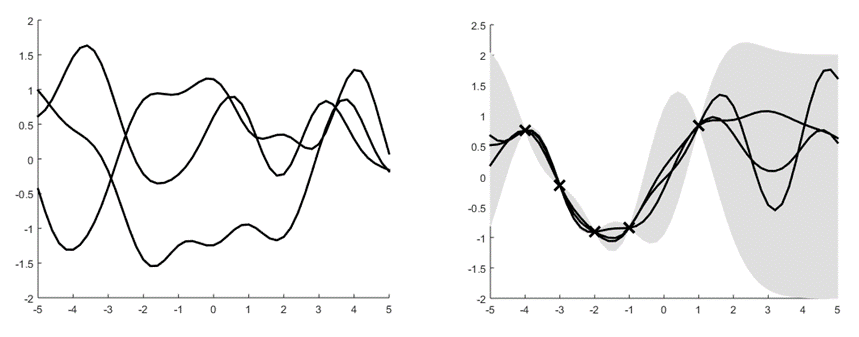
\includegraphics[width=0.8\textwidth, trim={10 10 10 10}]{figures/gp12.png}
    \caption{Gaussian process prior (left) and posterior (right).}
    \label{fig:gp12}
\end{figure}

Figure \ref{fig:gp12} shows three functions drawn at random from a GP prior (left) and GP posterior (right) after observing five data points in the case of noise-free observations. The shaded area corresponds to two times the standard deviation around the mean (95\% confidence region). We can see that the model perfectly interpolates the training data and that the predictive uncertainty increases as we move further away from the observed data.\\

Since our algorithm is defined in terms of inner products in the input space, it can be lifted into feature space by replacing the inner products with $k(x,x^{\prime})$, this is often referred to as the \textit{kernel trick}. The kernel measures similarity between objects and it doesn't require pre-processing them into feature vector format. For a example, a common kernel function is a \textit{radial basis function}:
\begin{equation}
    k(x,x^{\prime}) = \exp\bigg(-\frac{||x-x^{\prime}||^{2}}{2\sigma^2} \bigg)
\end{equation}
In the case of a Gaussian kernel, the feature map lives in an infinite dimensional space. In this case, it is clearly infeasible to explicitly represent the feature vectors. Another commonly used kernel in Gaussian process regression is the \textit{matern kernel}:
\begin{equation}
    \kappa(r) = \frac{2^{1-\nu}}{\Gamma(\nu)}\bigg(\frac{\sqrt{2\nu}r}{l}\bigg)^{\nu}K_{\nu}\bigg(\frac{\sqrt{2\nu}r}{l}\bigg)   
\end{equation}
where $r=||x-x^{\prime}||$, $\nu > 0$, $l > 0$, and $K_{\nu}$ is a modified Bessel function. As $\nu \rightarrow \infty$, this approaches the squared exponential kernel, if $\nu = \frac{1}{2}$, the kernel simplifies to $\kappa(r) = \exp(-r/l)$.\\

Assuming the observations are noisy, $y=f(x)+\epsilon$, where $\epsilon \sim N(0,\sigma_{y}^{2})$, GP is not required to interpolate the data but rather it must be close to the observed data. The covariance of the observed noisy responses is $\mathrm{cov}(y|X) = K + \sigma_{y}^{2}I = K_{y}$, where we assumed that the noise terms were independently added to each observation. Hence, the posterior predictive density is:
\begin{eqnarray}
    p(f_{\ast}|X_{\ast}, X, y) &\sim& N(f_{\ast}|\mu_{\ast},\Sigma_{\ast})\\
    \mu_{\ast} &=& K_{\ast}^{T}K_{y}^{-1}y\\
    \Sigma_{\ast} &=& K_{\ast\ast} - K_{\ast}^{T}K_{y}^{-1}K_{\ast}
\end{eqnarray}
In multiple dimensions, we can write down the \textit{square exponential kernel} as follows:
\begin{equation}
    \kappa_{y}(x_p, x_q) = \sigma_{f}^{2}\exp\big(-\frac{1}{2}(x_p-x_q)^{T}M(x_p-x_q)\big) + \sigma_{y}^{2}\delta_{pq}
\end{equation}
where $M = l^{-2}I$, $l$ is the horizontal scale over which the function changes, $\sigma_{f}^{2}$ controls the vertical scale and $\sigma_{y}^{2}$ is the observation noise variance. 

\begin{figure}[tbhp]
    \centering
    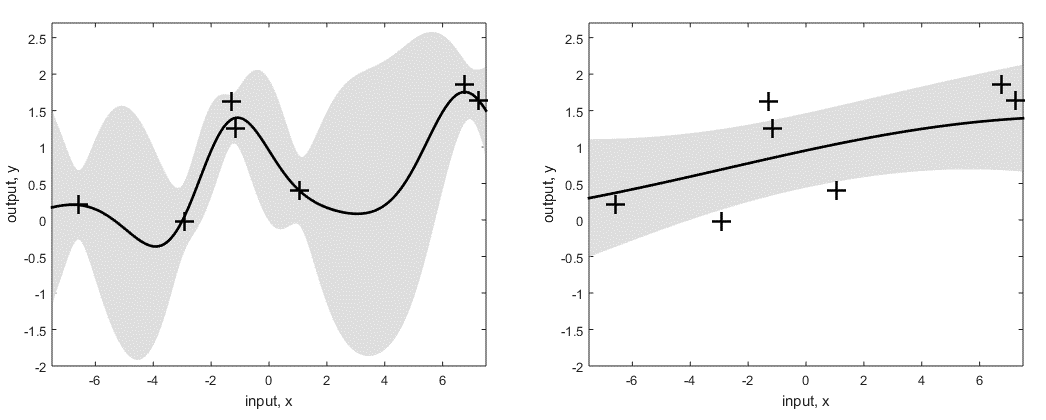
\includegraphics[width=0.8\textwidth, trim={10 10 10 10}]{figures/gp34.png}
    \caption{The effect of varying GP hyperparameters}
    \label{fig:gp34}
\end{figure}
Figure \ref{fig:gp34} shows the importance of choosing kernel hyperparameters and their impact  on GP regression. We fix $\sigma_{f}^{2} = 1$ and plot GP regression after $7$ noisy observations. On the left, the length scale and noise variance were set to $(l,\sigma_{y}^{2}) = (1, 0.2)$. We can see that the mean function appears wiggly and has a small bias due to observation noise. On the right, the kernel parameters were set to $(l,\sigma_{y}^{2}) = (10,0.8)$. The curve is much smoother due to large $l$ and also shows higher observation noise. 

Gaussian Processes (GPs) can be used for classification if the output of a GP is mapped to the range $[0, 1]$. In the binary case, we define the model as $p(y_i|x_i) = \sigma(f(x_i))$, where we let $\sigma(z)=(1+\exp(-z))^{-1}$. As with Bayesian logistic regression, the main difficulty in fitting GP classifier is that the Gaussian prior is not conjugate to the multinoulli likelihood. As a result several approximation algorithms can be used: Gaussian approximation, Expectation Propagation, variational and MCMC. 


\subsection{Dirichlet Process}


The Dirichlet process is a stochastic process used in Bayesian non-parametric models. Each draw from a Dirichlet process is a discrete distribution. For a random distribution $G$ to be distributed according to a DP, its finite dimensional marginal distributions have to be Dirichlet distributed. Let $H$ be a distribution over $\Theta$ and $\alpha$ be a positive real number. We say that $G$ is a Dirichlet process distributed with \textit{base distribution} $H$ and \textit{concentration parameter} $\alpha$ if:

\begin{equation}
    (G(A_1),...,G(A_r)) \sim \mathrm{Dir}(\alpha H(A_1),...,\alpha H(A_r))
\end{equation}
for every finite measurable partition $A_1$,...,$A_r$ of $\Theta$, where Dirichlet distribution is defined as:
\begin{equation}
    p(x_1,...,x_K) = \frac{\Gamma(\sum_k \alpha_k)}{\prod_k \Gamma(\alpha_k)}\prod_{k=1}^{K}x_{k}^{\alpha_k-1}
\end{equation}
The base distribution is the mean of the DP: $E[G(A)] = H(A)$, whereas the concentration parameter is the inverse variance: $V[G(A)] = H(A)(1-H(A))/(\alpha+1)$ for any measureable set $A\subset \Theta$. The larger the $\alpha$, the smaller the variance, and the DP will concentrate more of its mass around the mean.
\begin{figure}[tbhp]
    \centering
    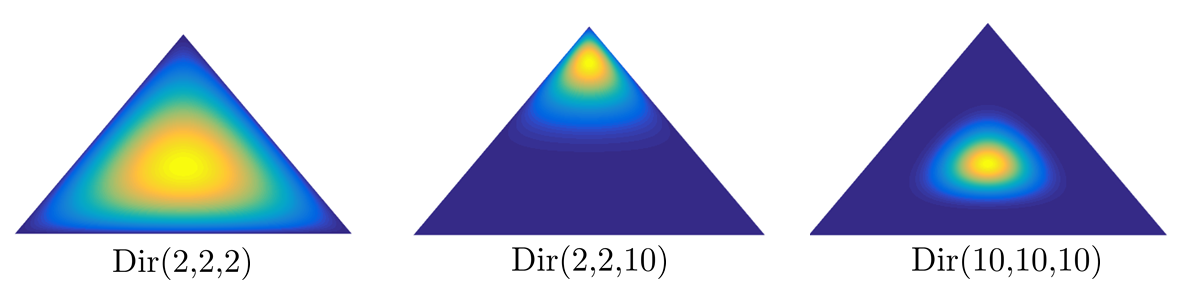
\includegraphics[width=0.8\textwidth, trim={10 10 10 10}]{figures/dir_merged.png}
    \caption{Dirichlet distribution: $\mathrm{Dir}(\alpha_1,\alpha_2,\alpha_3)$ over the simplex.}
    \label{fig:dir_merged}
\end{figure}
Let $\theta_1,...,\theta_n$ be a sequence of independent draws from $G\sim DP(\alpha,H)$. We are interested in the posterior distribution of G given observed values of $\theta_1,...,\theta_n$. Let $n_k$ be the number of observed values in $A_k$, the by conjugacy the Dirichlet and multinomial distributions we have:
\begin{equation}
    (G(A_1),...,G(A_r))|\theta_1,...,\theta_n \sim \mathrm{Dir}(\alpha H(A_1)+n_1,...,\alpha H(A_r)+n_r)
\end{equation}
The posterior is also a DP with an updated concentration parameter and base distribution \cite{Teh2010a}:
\begin{equation}\label{equ:dp_posterior}
    G|\theta_1,...,\theta_n \sim DP(\alpha+n, \frac{\alpha}{\alpha+n}H + \frac{n}{\alpha+n}\frac{\sum_{i=1}^{n}\delta_{\theta_i}}{n})
\end{equation}
Note that the posterior base distribution is a weighted average between the prior base distribution $H$ and the empirical distribution $\frac{1}{n}\sum_{i=1}^{N}\delta_{\theta_i}$. Therefore, $\alpha$ can be interpreted as the strength of the prior. 

\subsection{Construction of the DP}

The Dirichlet Process can be represented in different ways and the representation influences the inference procedure.

\subsubsection{Blackwell-MacQueen Urn Scheme}

The Blackwell-MacQueen Urn Scheme, also commonly known as the Polya urn scheme, provides a way of constructing a sequence of draws $\theta_1, \theta_2,...,\theta_n~\sim G$ where $G\sim DP(\alpha, H)$ without explicitly having to represent $G$. The posterior distribution with $G$ marginalized out and $\theta_1 \sim H$ can be written as:
\begin{equation}\label{equ:urn}
    \theta_{n+1}|\theta_1,...,\theta_n \sim \frac{1}{\alpha+n}\bigg(\alpha H + \sum_{i=1}^{n}\delta_{\theta_i}\bigg)
\end{equation}
The above equation describes a sequential process for drawing $\theta_i$ from $G$, which can be described by the following urn metaphor. First draw $\theta_1 \sim H$, paint a ball with that color and put it in the urn. Then, at each subsequent step $n$, either draw $\theta_n \sim H$ with probability $\alpha/(\alpha + n)$ and put a ball of that color in the urn, or with probability $n/(\alpha + n)$, randomly draw a ball from the urn, set $\theta_n$ to its color, then paint a new ball in that color and return both balls to the urn.

\begin{figure}[tbhp]
    \centering
    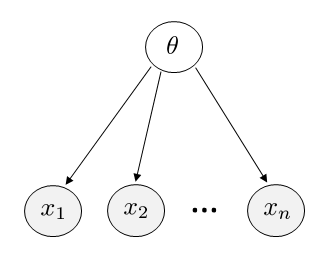
\includegraphics[width=0.3\textwidth, trim={10 10 10 10}]{figures/naive_bayes_gm.png}
    \caption{Naive Bayes graphical model}
    \label{fig:naive_bayes_gm}
\end{figure}

The Blackwell-MacQueen urn model has been used to show the existence of the DP. Starting from (\ref{equ:urn}) we can construct a distribution over draws as follows:
\begin{equation}
    P(\theta_1,...,\theta_n) = \prod_{i=1}^{n}P(\theta_i|\theta_1,...,\theta_{i-1})
\end{equation}
This random sequence is infinitely exchangeable: the probability of generating $\theta_1,...\theta_n$ in that order is equal to the probability of generating them in any alternative order. Thus, for a given permutation $\sigma$, we have
\begin{equation}
    P(\theta_1,...,\theta_n) = P(\theta_{\sigma(1)},...,\theta_{\sigma(2)})
\end{equation}
The strength of infinite exchangeability lies in the following theorem:
\begin{theorem}
(De Finetti, 1930s) A sequence of random variables $x_1, x_2,..,x_n$ is infinitely exchangeable iff for all $n$:
\begin{equation}
    p(x_1,x_2,...,x_n) = \int p(\theta)\prod_{i=1}^{n}p(x_i|\theta)d\theta
\end{equation}
\end{theorem}
Therefore, if we have exchangeable data, there must exist a parameter $\theta$, a likelihood $p(x|\theta)$ and a distribution $P$ on $\theta$ such that conditioned on $\theta$ the observations are independent as shown in Figure \ref{fig:naive_bayes_gm}. In our setting, the prior over the random distribution $p(\theta)$ is the Dirichlet Process $DP(\alpha, H)$, thus establishing existence.

\subsubsection{Chinese Restaurant Process}

Chinese Restaurant Process (CRP) is a discrete-time stochastic process that is based on the clustering property of a DP. Let $\theta_{1}^{\ast},...,\theta_{m}^{\ast}$ be unique values of draws $\theta_1,...,\theta_n$ and $n_k$ be the number of repetitions of $\theta_{k}^{\ast}$. Then, the predictive distribution can be written as:
\begin{equation}
    \theta_{n+1}|\theta_1,...,\theta_n \sim \frac{1}{\alpha+n}\bigg(\alpha H + \sum_{k=1}^{m}n_k \delta_{\theta_{k}^{\ast}}\bigg)
\end{equation}
Notice that $\theta_{k}^{\ast}$ will be repeated in proportion to $n_k$, the number of times it has already been observed. This is a \textit{rich-gets-richer} phenomenon: the larger the cluster, the faster it will grow.
The Chinese Restaurant Process takes its name from a metaphor describing its construction: imagine a Chinese restaurant which has an infinite number of tables, each of which can accomodate an infinite number of clusters. The first customer enters the restaurant and sits at the first table. The $n+1$st customer either joins an already occupied table $k$ with probability proportional to $n_k$ of customers already there or sits at a new table with probability proportional to $\alpha$. Representing customers with integers and tables with clusters, CRP defines a partition on $[n]$. The number of occupied tables $K$ approaches $\alpha \log(n)$ as $n$ approaches infinity. And therefore, DP is a non-parametric prior that favors models whose complexity grows with the amount of data.   

\subsubsection{Stick-Breaking Construction}

The stick breaking construction \cite{sethuraman94} represents draws $G\sim DP(\alpha, H)$ as a weighted sum of atoms (point masses). It is given as follows:
\begin{eqnarray}
    \beta_k \sim \mathrm{Beta}(1,\alpha) ~~~ ~~~~ ~~~~ ~~~~ \theta_{k}^{\ast}\sim H\\
    \pi_k = \beta_k\prod_{l=1}^{k-1}(1-\beta_l) ~~~~ ~~~~ G = \sum_{k=1}^{\infty}\pi_k \delta_{\theta_{k}^{\ast}}
\end{eqnarray}

\begin{figure}[tbhp]
    \centering
    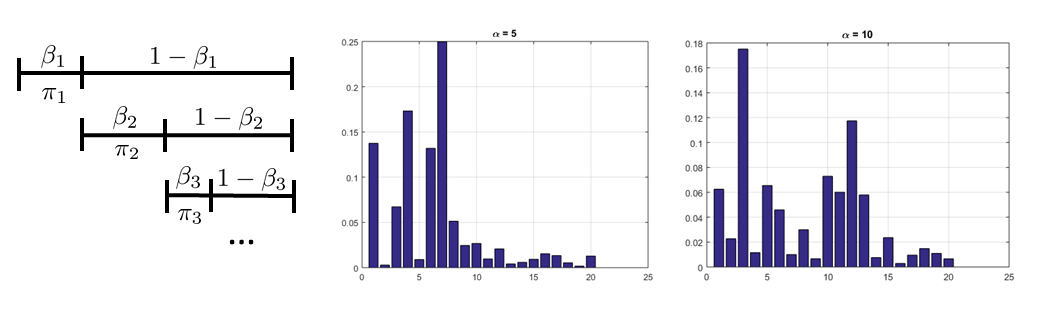
\includegraphics[width=0.8\textwidth, trim={10 10 10 10}]{figures/stick_breaks.png}
    \caption{Stick-Breaking Weights}
    \label{fig:sticks}
\end{figure}

This construction guarantees that $G\sim DP(\alpha, H)$. The name stick-breaking comes from the fact that one can interpret the $\pi_k$ as the lengths broken off a unit length stick as shown in Figure \ref{fig:sticks} for $\alpha=5$ and $\alpha=10$.

\subsection{Hierarchical Dirichlet Process (HDP)}


Hierarchical Dirichlet Processes model problems involving groups of data, where each observation within a group is a draw from a mixture model and mixture components are shared between groups. In each group, the number of components is learned from data using a Dirichlet Process prior. In addition, the base measure for the child Dirichlet processes is itself distributed according to a Dirichlet process. Since a draw from the global DP is a discrete distribution, the group-level DPs share mixture components. 
The HDP model can be summarized as follows and is shown in Figure \ref{fig:hdp_gm}:
\begin{eqnarray}
   G_0 | \gamma, H \sim DP(\gamma, H)\\
   G_j | \alpha, G_0 \sim DP(\alpha, G_0)
\end{eqnarray}
\begin{figure}[tbhp]
    \centering
    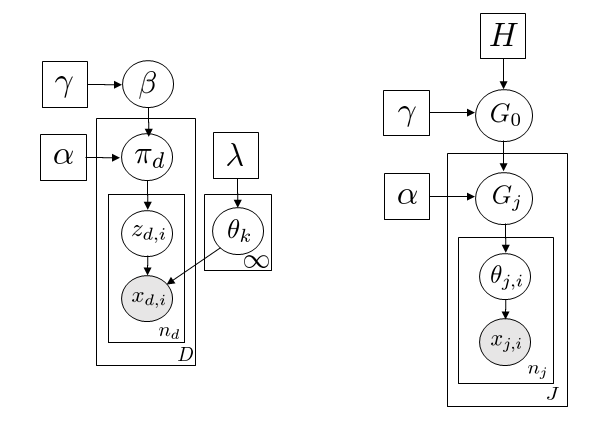
\includegraphics[width=0.6\textwidth, trim={10 10 10 10}]{figures/hdp_gm.png}
    \caption{HDP Graphical Model}
    \label{fig:hdp_gm}
\end{figure}
The distribution $G_0$ varies around the prior $H$, with the amount of variability given by $\gamma$. The actual distribution $G_j$ over $\theta_{j,i}$ in $j^{th}$ group deviates from $G_0$ with the amount of variability given by $\alpha$. If we expect the amount of variability between groups to be different, we can use a separate concentration parameter $\alpha_j$ for each group $j$.\\

Given the global DP prior $G_0$, we can express it using a stick-breaking representation:
$G_0 = \sum_{k=1}^{\infty}\beta_k \delta_{\phi_k}$, where $\phi_k \sim H$ and $\beta_k \sim \mathrm{GEM}(\gamma)$. Since $G_0$ has support at the points $\phi_k$, each $G_j$ has support at these points as well and can be written as: $G_j = \sum_{k=1}^{\infty}\pi_{jk}\delta_{\phi_k}$. The group weights $\pi_j$ are related to global weights $\beta$ as follows \cite{teh2005jasa}:

\begin{eqnarray}
    \beta_{k}^{\prime} \sim \mathrm{Beta}(1,\gamma) ~~~~~~~~ \beta_k = \beta_{k}^{\prime}\prod_{l=1}^{k-1}(1-\beta_{l}^{\prime})\\
    \pi_{jk}^{\prime} \sim \mathrm{Beta}(\alpha\beta_k, \alpha(1-\sum_{l=1}^{k}\beta_l)) ~~~~~~~~ \pi_{jk} = \pi_{jk}^{\prime}\prod_{l=1}^{k-1}(1-\pi_{jl}^{\prime})
\end{eqnarray}

An analog of the Chinese restaurant process for HDPs is the Chinese restaurant franchise (CRF): the metaphor is extended to allow multiple restaurants which share a set of dishes. In this interpretation, each group defines a separate restaurant in which customers (observations) $x_{ji}$ sit at tables (clusters) $t_{ji}$. Each table shares a single dish (parameter) $\theta_{ji}$, which is ordered from a menu $G_0$ shared among restaurants (groups) as shown in Figure \ref{fig:crf}\\
\begin{figure}[thpb]
    \centering
    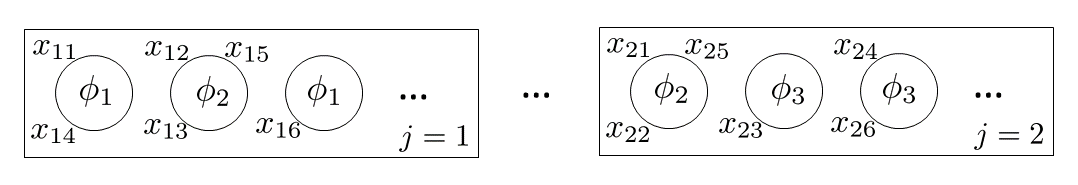
\includegraphics[width=0.8\textwidth, trim={10 10 10 10}]{figures/crf.png}
    \caption{Chinese Restaurant Franchise (CRF). Each restaurant is represented by a rectangle. Customers $x_{ji}$ are seated at tables. At each table a dish $\phi_k$ is served from a global menu.}
    \label{fig:crf}
\end{figure}

Let $\phi_1,...,\phi_K$ denote the $K$ atoms distributed according to $H$: this is the global menu of dishes. Let $\psi_{jt}$ represent table-specific choice of dishes; in particular $\psi_{jt}$ is the dish served at table $t$ in restaurant $j$. Note that each $\theta_{ji}$ is associated with one $\psi_{jt}$ and each $\psi_{jt}$ is associated with one $\phi_k$. In the CRF metaphor, customer $i$ in restaurant $j$ sat at table $t_{ji}$, while table $t$ in restaurant $j$ served dish $k_{jt}$.

The number of tables in restaurant $j$ serving dish $k$ is denoted $m_{jk}$, and the number of customers in restaurant $j$ at table $t$ eating dish $k$ is $n_{jtk}$. Marginal counts are represented with dots. For example, $n_{j..}$ and $m_{j.}$ represent the number of customers and tables, respectively, in restaurant $j$.\\

We can compute the marginals under HDP when $G_0$ and $G_j$ are integrated out using (\ref{equ:dp_posterior}):
\begin{equation}\label{equ:hdp_theta}
    \theta_{ji}|\theta_{j1},...,\theta_{jn},\alpha,G_0 \sim \sum_{t=1}^{m_{j.}} \frac{n_{jt.}}{n+\alpha}\delta_{\psi_{jt}} + \frac{\alpha}{n+\alpha}G_0
\end{equation}
If a term in the first summation is chosen, we set $\theta_{ji}=\psi_{jt}$. If the second term is chosen then we increment $m_{j.}$ by one and draw $\psi_{jm_{j.}}\sim G_0$. To integrate out $G_0$, we can use (\ref{equ:dp_posterior}) again:
\begin{equation}\label{equ:hdp_psi}
    \psi_{jt}|\psi_{11},\psi_{12},...,\psi_{21},...,\gamma,H \sim \sum_{k=1}^{K}\frac{m_{.k}}{m_{..}+\gamma}\delta_{\phi_k} + \frac{\gamma}{m_{..}+\gamma}H
\end{equation}
To summarize, for each $j$ and $i$, we first sample $\theta_{ji}$  using (\ref{equ:hdp_theta}). If a new sample from $G_0$ is needed, we use (\ref{equ:hdp_psi}) to obtain a new sample $\psi_{jt}$.

An on-line variational inference algorithm for Hierarchical Dirichlet Process \cite{wang11a} was used to fit a topic model on the 20newsgroups dataset. The dataset consists of $11,314$ documents and over $100K$ unique tokens. Standard text pre-processing was used including tokenization, stop-word removal and stemming. A compressed dictionary of $4K$ words was constructed by filtering out tokens that appear in less than $5$ documents and more than $50\%$ of the corpus. The top-level truncation was set to $T=20$ topics and the second level truncation was set to $K=8$ topics. The concentration parameters were chosen as $\gamma = 1.0$ at the top-level and $\alpha=0.1$ at the group level to yield a broad range of shared topics that are concentrated at the group level. Figure \ref{fig:hdp_topics} shows a sample of the global level topics inferred by online variational HDP algorithm. We can find topics about autos, politics and for sale items that correspond to the target labels of the 20newsgroups dataset.
\begin{figure}[thpb]
    \centering
    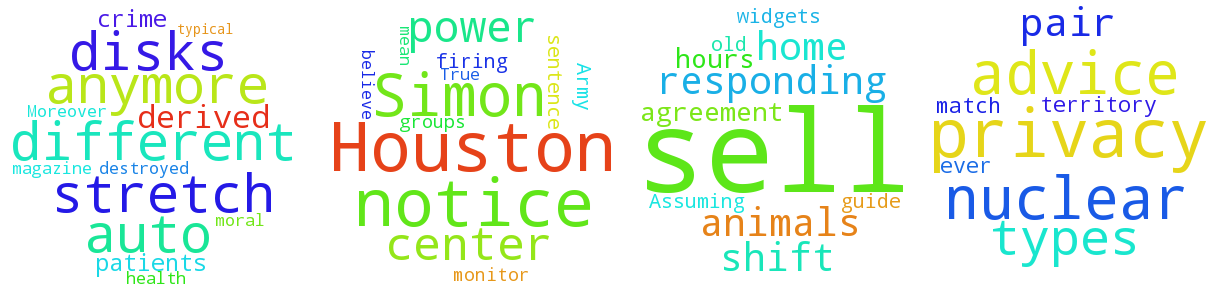
\includegraphics[width=0.8\textwidth, trim={10 10 10 10}]{figures/hdp_topics.png}
    \caption{Sample of HDP topics inferred using online variational bayes algorithm on 20newsgroups dataset.}
    \label{fig:hdp_topics}
\end{figure}

\subsubsection{HDP Hidden Markov Models}

The Hierarchical Dirichlet Process (HDP) can be used to define a prior distribution on transition matrices over countably infinite state spaces. The HDP-HMM is known is an infinite Hidden Markov Model where the number of states is inferred automatically. To consider a non-parametric variant of the HMM, we must consider a set of DPs, one for each value of the current state. In addition, the DPs must be linked because we want the same set of next states to be reachable from each of the current states. The relates directly to HDP, where the atoms associated with state-conditional DPs are shared.

\begin{figure}[thpb]
    \centering
    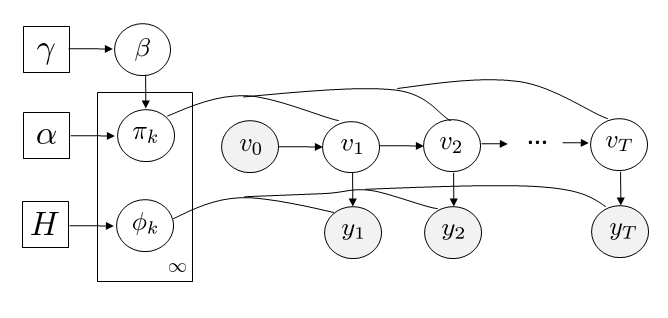
\includegraphics[width=0.6\textwidth, trim={10 10 10 10}]{figures/hdp_hmm_gm.png}
    \caption{HDP-HMM graphical model}
    \label{fig:hdp_hmm_gm}
\end{figure}

We can describe the HDP-HMM model in Figure \ref{fig:hdp_hmm_gm} using the stick-breaking construction. The parameters have the following distribution:
\begin{equation}
    \beta|\gamma \sim \mathrm{GEM}(\gamma) ~~ \pi_k|\alpha,\beta \sim DP(\alpha,\beta) ~~ \phi_k|H \sim H
\end{equation}
for each $k=1,2,...$ while for time steps $t=1,...,T$ the state and observation distributions are:
\begin{equation}
    v_t|v_{t-1}, \pi_k \sim \pi_{v_{t-1}} ~~~~ y_t|v_{t},\phi_k \sim F(\phi_{v_t})
\end{equation}
given a starting state $v_0$. Each $\pi_j$ is a DP draw and is interpreted as the transition distribution from state $j$. The $\pi_j$s are linked through DP draws parameterized by the same discrete measure $\beta$. Therefore, the states are shared between different DP draws. 

Besides Gibbs sampling, one way to compute the posterior for infinite HMM is using a \textit{beam sampling} algorithm \cite{VanSaaTeh2008a}. Beam sampling combines two ideas: slice sampling and dynamic programming to sample whole state trajectories. Slice sampling is applied to limit the number of states to a finite number in each time step of the iHMM. The underlying idea is to limit the beam search to a small number of states so that a good trajectory can be found. Beam sampling is an MCMC method that guarantees convergence to the true posterior.\\

\begin{figure}[thpb]
    \centering
    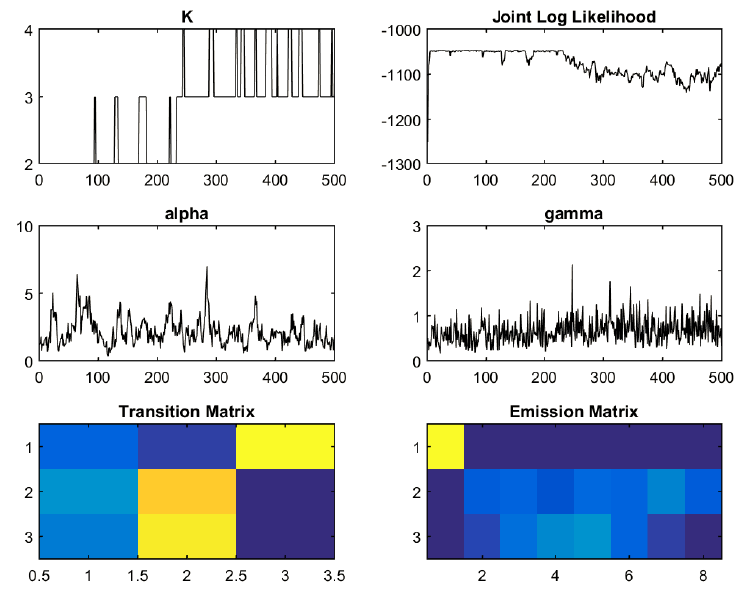
\includegraphics[width=0.7\textwidth, trim={10 10 10 10}]{figures/ihmm_beam.png}
    \caption{HDP-HMM inference results using the beam sampling algorithm \cite{VanSaaTeh2008a}.}
    \label{fig:ihmm_beam}
\end{figure}

Figure \ref{fig:ihmm_beam} shows posterior inference results for synthetically generated time-series data. The ground truth data was generated using $4$ unique states for given transition and emition matrices. From the top-left plot in Figure \ref{fig:ihmm_beam}, we can see that the beam sampler discovered three transition states at iteration $250$. We can also see the samples of $\alpha$ and $\gamma$ concentration parameters for the HDP-HMM as well as the transition and emission matrices. 


\subsection{Dependent Dirichlet Process (DDP)}


The earlier part of Bayesian non-parametric literature focused on problems where a single distribution is assigned a non-parametric prior. However, in many applications, the objective is modelling a collection of distributions used in temporal and spatial processes. The Dirichlet process assumes that observations are exchangeable and therefore the data points have no inherent ordering that influences their labelling. This assumption is invalid for modelling termporal and spatial processes in which the order of data points plays a critical role in creating meaningful clusters.\\

The dependent Dirichlet process (DDP) originally formulated by MacEachern \cite{maceachern99a} provides a non-parametric prior over evolving mixture models. A construction of the DDP built on Poisson process \cite{dhlin10nips} led to the development of the DDP mixture model (DDPMM) which generalizes DPMM by including birth, death and transition processes for the clusters in the model. In addition, a low-variance approximations to DDPMM have been derived leading to a dynamic clustering algorithm \cite{Campbell13_NIPS}.\\

\begin{figure}[thpb]
    \centering
    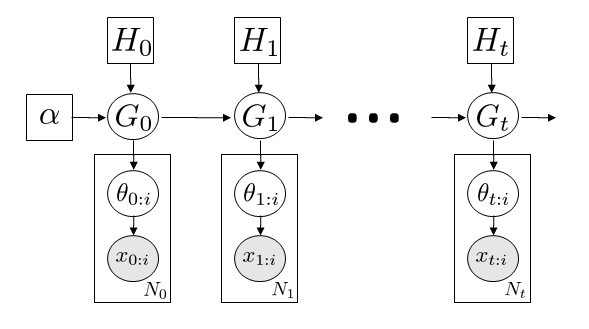
\includegraphics[width=0.6\textwidth, trim={10 10 10 10}]{figures/ddp_gm.png}
    \caption{Dependent Dirichlet Process (DDP) graphical model.}
    \label{fig:ddp_gm}
\end{figure}

Under time-varying setting, it is natural to introduce different DP priors for different time steps as shown in Figure \ref{fig:ddp_gm}. The generative model can be written as:
\begin{eqnarray}
    D_t \sim DP(\alpha, H_t)\\
    \theta_{t:i}|D_t \sim D_t ~~~for i=1,...,n_t,~t=0,...,T\\
    x_{t:i}|\theta_{t:i} \sim F(\theta_{t:i}) ~~~for i=1,...,n_t,~t=0,...,T
\end{eqnarray}

A Poisson-based construction of DDP \cite{dhlin10nips} exploits the connection between Poisson and Dirichlet processes. In particular, by applying operations that preserve \textit{complete randomness} to the underlying Poisson processes: superposition, subsampling and point transition, a new Poisson and therefore a new Dirichlet process is produced. Therefore, a Markov chain of Dirichlet processes can be written as:
\begin{equation}
    D_t = T(S_q(D_{t-1}))\bigoplus H_t, ~~~where H_t \sim DP(\alpha, H)
\end{equation}
where $S_q$ is an acceptance function, $T$ is a probabilistic transition, combined with new terms from innovation process $H_t$ to form $D_t$. 


\subsection{Indian Buffet Process}

The Indian Buffet Process(IBP) is a stochastic process defining a probability distribution over sparse binary matrices with a finite number of rows and an infinite number of columns. This distribution is suitable to use as a prior for models with potentially infinite number of features. The form of the prior ensures that only a finite number of features will be present in any finite set of observations but more features may appear as more data points are observed.\\

Let $Z$ be a $N\times K$ binary matrix indicating the presence or absence of a latent feature. The IBP places the following prior on $Z$ \cite{ibp2011}:
\begin{equation}
    p(Z) = \frac{\alpha^K}{\prod_{i=1}^{N}K_{1}^{(i)}!}\exp\{-\alpha H_N\}\prod_{k=1}^{K}\frac{(N-m_k)!(m_k-1)!}{N!}
\end{equation}
where $K$ is the number of nonzero columns in $Z$, $m_k$ is the number of ones in column $k$ of $Z$, $H_N$ is the $N^{th}$ harmonic number, and $K_h$ is the number of occurences of the non-zero binary vector $h$ among the columns in $Z$. The parameter $\alpha$ controls the expected number of features present in each observation.\\

In the Indian Buffet Process (IBP), the rows of $Z$ correspond to customers and the columns correspond to dishes in an infinitely long buffet. The first customer takes the first $\mathrm{Poisson}(\alpha)$ dishes. The $i$th customer than takes dishes that have been previously sampled with probability $m_k/i$, where $m_k$ is the number of people who have already sampled dish $k$. He also takes $\mathrm{Poisson}(\alpha/i)$ new dishes. Then, $z_{nk}$ is one if customer $n$ tried $k$th dish and zero otherwise.

\begin{figure}[thpb]
    \centering
    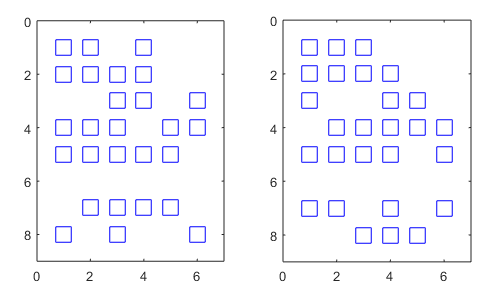
\includegraphics[width=0.5\textwidth, trim={10 10 10 10}]{figures/lof_feature_matrix.png}
    \caption{Original binary feature matrix (left) and its left-ordered form (right)}
    \label{fig:lof}
\end{figure}

This process is infinitely exchangeable for an equivalence class of binary matrices defined by a left-ordered many-to-one function. $lof(Z)$ is obtained by ordering the columns of the binary matrix $Z$ from left to right by the magnitude of the binary number expressed by that column, taking the first row as the most significant bit. The left ordering of a binary matrix is shown in Figure \ref{fig:lof}\\

In this section, we focus on variational inference procedures for the linear-Gaussian likelihood model \cite{DosMilVan2009a}. Let $X$ be a $N\times D$ matrix where each of the $N$ rows contains a $D$-dimensional observation. We focus on a model where $X$ can be approximated as:
\begin{equation}
    X_{N\times D} = Z_{N\times K} \times A_{K\times D} + \epsilon
\end{equation}
where $Z$ is a binary feature matrix, the values for feature $k$ are stored in row $k$ of $A$, and $\epsilon$ is measurement noise.
\begin{figure}[thpb]
    \centering
    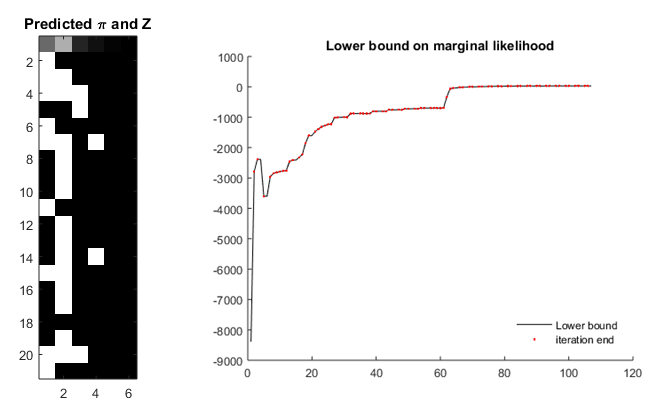
\includegraphics[width=0.6\textwidth, trim={10 10 10 10}]{figures/ibp_z.png}
    \caption{Predicted IBP binary feature matrix $Z$ using variational inference.}
    \label{fig:ibp_z}
\end{figure}
Figure \ref{fig:ibp_z} shows the predicted binary feature matrix $Z$ and lower bound on marginal likelihood using variational inference algorithm for IBP \cite{DosMilVan2009a}. The concentration parameter was set to $\alpha=1$ and the feature truncation level was set to $K=6$. 



\subsection{DPMM}

The Dirichlet Process Mixture Models (DPMM) belong to a class of \textit{infinite mixture models}, in which we do not impose any prior knowledge on the number of clusters $K$. DPMM models learn the number of clusters from the data using a non-parametric prior based on the Dirichlet Process (DP). Automatic model selection leads to computational savings of cross validating the model for multiple values of $K$.\\

Consider the graphical model of the DPMM in Figure \ref{fig:dpmm_gm}.
\begin{figure}[thpb]
    \centering
    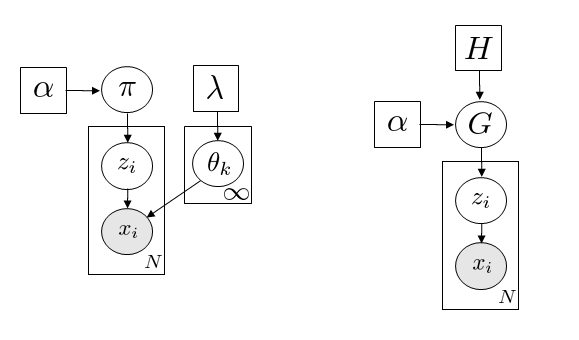
\includegraphics[width=0.6\textwidth, trim={10 10 10 10}]{figures/dpmm_gm.png}
    \caption{DPMM Graphical Model}
    \label{fig:dpmm_gm}
\end{figure}
For each data point $x_i$, there's a corresponding label $z_i$ that assigns the point to one of the clusters with mixture weight $\pi_k$ and parameters $\theta_k = \{\mu_k, \Sigma_k\}$. The generative model can be written as follows:
\begin{eqnarray}
    p(x_i|z_i=k,\theta) &=& p(x_i|\theta_k) \\
    p(z_i=k|\pi) &=& \pi_k \\
    p(\pi|\alpha) &=& \mathrm{Dir}(\pi|\alpha) \\
    p(\theta_k|\beta) &=& \mathrm{NIW}(\mu_k,\Sigma_k|m_0,\kappa_0,\nu_0,S_0)
\end{eqnarray}
An equivalent representation of this model can be written as:
\begin{eqnarray}
    G(\theta) = \sum_{k=1}^{\infty}\pi_k \delta_{\theta_k}
\end{eqnarray}
where $\pi \sim \mathrm{Dir}(\alpha_1,...,\alpha_K)$ and $\theta_k \sim H$. Therefore, $G$ is an infinite mixture of cluster functions of delta functions. In practice, we can construct $G$ using a \textit{stick-breaking construction}:
\begin{eqnarray}
    \beta_k \sim \mathrm{Beta}(1,\alpha)\\
    \pi_k = \beta_k \prod_{l=1}^{k-1}(1-\beta_l) = \beta_k(1-\sum_{l=1}^{k-1}\pi_l)
\end{eqnarray}
This is commonly denoted as $\pi \sim \mathrm{GEM}(\alpha)$. The number of generated mixture components increases with $\alpha$. The hyper-parameter $\alpha$ controls the expected number of clusters:
\begin{eqnarray}
    E[K] = \alpha \times \log(1+n/\alpha)\\
    VAR[K] = \alpha \times \log(1+n/\alpha)
\end{eqnarray}
Thus, the number of clusters grows logarithmically with the number of data points and in direct proportion to $\alpha$ as shown in Figure \ref{fig:dpmm_merged1} 
\begin{figure}[thpb]
    \centering
    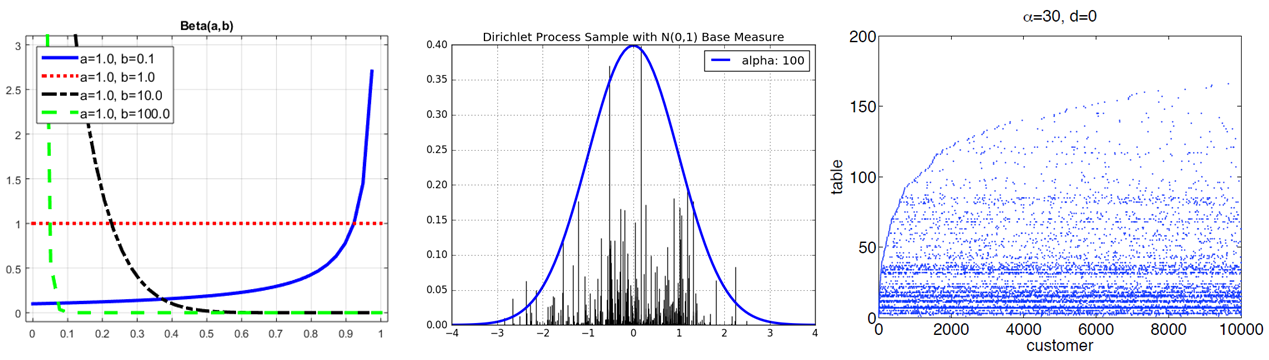
\includegraphics[width=0.9\textwidth, trim={10 10 10 10}]{figures/dp_merged1.png}
    \caption{a) $\mathrm{Beta}(1,\alpha)$ b)DP samples c) DP cluster growth }
    \label{fig:dpmm_merged1}
\end{figure}

\subsection{Fitting a DPMM model}

One way to fit a DPMM is to modify the collapsed Gibbs sampler for a finite mixture model \cite{MurphyML}:
\begin{equation}
    p(z_i=k|z_{-i},x,\alpha,\beta) \propto p(z_i=k|z_{-i},\alpha)p(x_i|x_{-i},z_i=k,z_{-i},\beta)
\end{equation}
The first term is given by the Chinese Restaurant Process (CRP):
\begin{equation}
    p(z_i=k|z_{-i},\alpha) = 
    \begin{cases}
        \frac{N_k}{N+\alpha -1} & \text{if } k \text{ is occupied}\\
        \frac{\alpha}{N+\alpha-1} & \text{if } k \text{ is a new cluster}
    \end{cases}
\end{equation}
The second term is the posterior predictive and can be computed as follows:
\begin{equation}
    p(x_i|x_{-i},z_i=k,z_{-i},\beta) = p(x_i|x_{k\setminus i}, \beta) = \frac{p(x_{k}|\beta)}{p(x_{k\setminus i}|\beta)}
\end{equation}
We can compute both the numerator and the denominator above if we can find an expression for the marginal $p(x)$:
\begin{eqnarray}
    p(x) &=& \int_{\mu} \int_{\Sigma} p(x,\mu,\Sigma) d\mu d\Sigma = \int_{\mu} \int_{\Sigma} p(x|\mu,\Sigma)p(\mu,\Sigma|\beta)d\mu d\Sigma\\
    &=& (2\pi)^{-ND/2}\frac{Z_{NIW}(D,\kappa_N,\nu_N,S_N)}{Z_{NIW}(D,\kappa_0,\nu_0,S_0)} = \pi^{-ND/2}\frac{\kappa_{0}^{D/2}|S_0|^{\nu_0/2}}{\kappa_{N}^{D/2}|S_N|^{\nu_N/2}}\prod_{i=1}^{D}\frac{\Gamma(\frac{\nu_N+1-i}{2})}{\Gamma(\frac{\nu_0+1-i}{2})}
\end{eqnarray}
Therefore, we can write the second term as follows:
\begin{eqnarray}
    \log p(x_i|x_{k\setminus i}) = z(D,N+1,\kappa_{N+1},\nu_{N+1},S_{Ni}) - z(D,N,\kappa_{N},\nu_N,S_N)\\
    z(D,N,\kappa,\nu,S) = -\frac{ND}{2}\log \pi - \frac{D}{2}\log \kappa - \frac{\nu}{2}\log |S| + \sum_{i=1}^{D}\log \Gamma(\frac{\nu+i-1}{2})
\end{eqnarray}
We can summarize, the collapsed Gibbs sampler for an infinite Gaussian mixture model in Algorithm \ref{alg:dpmm_collapsed}.
\begin{algorithm}
\caption{Collapsed Gibbs for DPMM}
\label{alg:dpmm_collapsed}
\begin{algorithmic}[1]
\STATE Initialize labels $z$ 
\STATE for t = 1,2,...,T do 
\STATE ~~~ for i = 1,2,...,N do 
\STATE ~~~ ~~~ remove $x_i$'s statistics from component $z_i$ 
\STATE ~~~ ~~~ delete empty component
\STATE ~~~ ~~~ for k = 1,2,...,K+1 do
\STATE ~~~ ~~~ ~~~ compute $\log p(z_i=k|z_{-i},x,\alpha,\beta) \sim$
\STATE ~~~ ~~~ ~~~ $\log p(z_i = k|z_{-i},\alpha) + \log p(x_i|x_{k\setminus i},\beta)$
\STATE ~~~ ~~~ sample $z_i = k_{new}$ from $p(z_i=k|z_{-i},x,\alpha,\beta)$
\STATE ~~~ ~~~ create a new cluster if $z_i = K+1$
\STATE ~~~ ~~~ add $x_i$'s statistics to component $z_i = k_{new}$ 
\STATE ~~~ end for
\STATE end for
\end{algorithmic}
\end{algorithm}

Figure \ref{fig:dp_results} shows the clustering results of DPMM collapsed gibbs sampler with Gaussian base measure and $\alpha=1$ after $100$ iterations on a synthetic dataset of $1K$ points in 2D. The sampler was initialized with $K_{init}=2$ clusters and correctly identified all $5$ clusters in the data.

\begin{figure}[thpb]
    \centering
    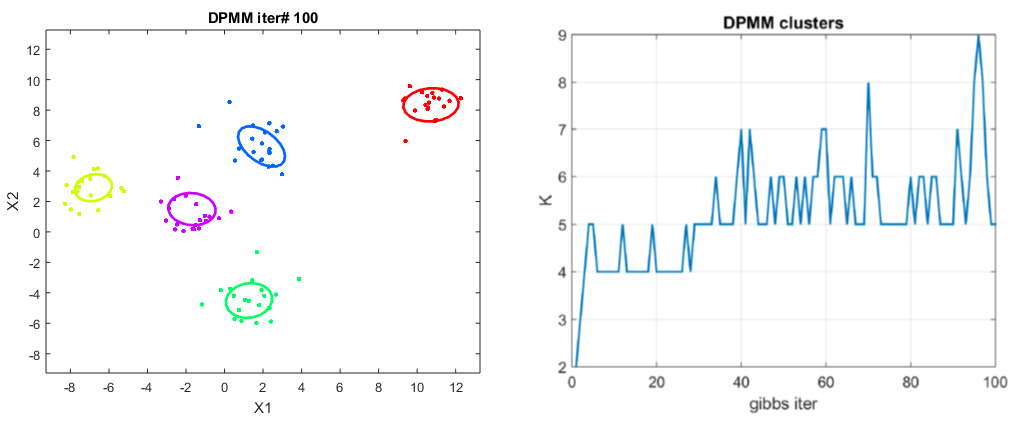
\includegraphics[width=0.8\textwidth, trim={10 10 10 10}]{figures/dp_results.png}
    \caption{DPMM Clustering Results for Gaussian data}
    \label{fig:dp_results}
\end{figure}

Figure \ref{fig:dp_results2} shows the clustering results of DPMM on categorical data. Documents from a reduced NIPS dataset with 300 docs, 5K vocab and 130K words were grouped into $11$ clusters. The top words for the first $4$ clusters are displayed in Figure \ref{fig:dp_results2}. The results indicate meaningful division of articles by topics about neural networks, gaussian mixtures, computer vision and reinforcement learning. The gibbs sampler was initialized with $K_{init}=2$ and $\alpha=1$ and coverged after $20$ iterations through the corpus.   

\begin{figure}[thpb]
    \centering
    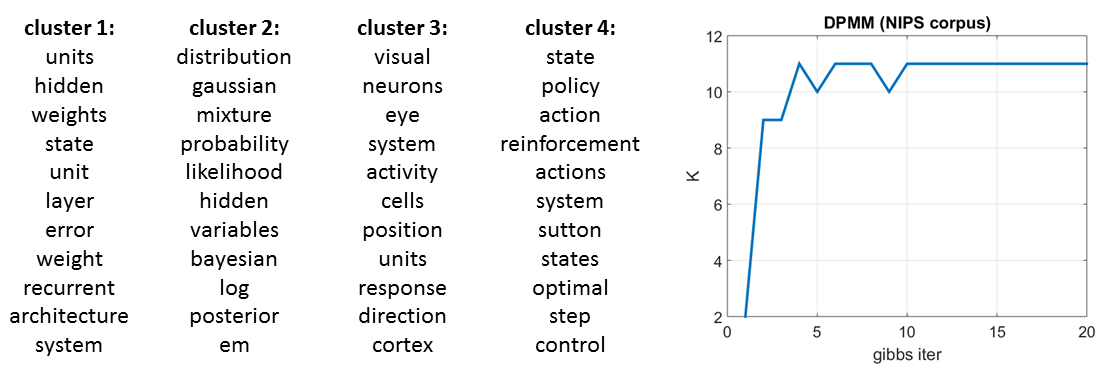
\includegraphics[width=0.8\textwidth, trim={10 10 10 10}]{figures/dp_results2.png}
    \caption{DPMM Clustering Results for Categorical data}
    \label{fig:dp_results2}
\end{figure}





\section{Variational Inference}
This section focuses on a class of approximate inference algorithms based on variational inference. The basic idea is to choose an approximation $q(x)$ from a tractable family of distributions and then make this approximation as close as possible to the true posterior $p^{\ast}(x)$. This reduces inference to an optimization problem.\\

We can use KL divergence to measure the distance between distributions. In particular, we use reverse KL to make the computation tractable.
\begin{equation}
    KL(q||p^{\ast}) = \sum_x q(x) \log \frac{q(x)}{p^{\ast}(x)}
\end{equation}
Let $\tilde{p}(x)=p^{\ast}(x)Z$ be the un-normalized distribution, then our objective function:
\begin{eqnarray}
    J(q) = KL(q||\tilde{p})= \sum_x q(x) \log \frac{q(x)}{p^{\ast}(x)Z} 
    = \sum_x q(x) \log \frac{q(x)}{p^{\ast}(x)} - \log Z = KL(q||p^{\ast}) - \log Z
\end{eqnarray}
Since KL divergence is non-negative, $J(q)$ is an upper bound on the marginal likelihood:
\begin{eqnarray}
    J(q) = KL(q||p^{\ast}) - \log Z \geq -\log Z = -\log p(D)
\end{eqnarray}
when $q(x)$ equals the true posterior $p^{\ast}(x)$, the KL divergence vanishes and the optimal value $J(q^{\ast})$ equals the log partition function and for all other values of $q$ it yields a bound. $J(q)$ is called the \textit{variational free energy} and can be written as:
\begin{equation}\label{equ:var_obj}
   \min_q J(q) = E_{q}[\log q(x)]+E_{q}[-\log \tilde{p}(x)] = -H(q) + E_q[E(x)]
\end{equation}
The variational objective function (\ref{equ:var_obj}) is closely related to energy minimization in statistical physics. The first term acts as a regularizer by encouraging maximum entropy, while the second term is the expected energy and encourages the variational distribution $q$ to explain the data. 

\begin{figure}[tbhp]
    \centering
    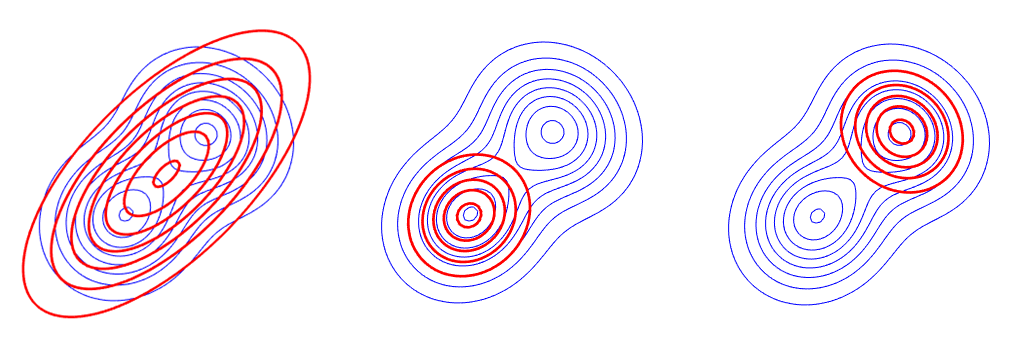
\includegraphics[width=0.7\textwidth, trim={10 10 10 10}]{figures/kl_bimodal.png}
    \caption{Forward vs reverse KL on a bimodal distribution. The blue contours is the true distribution $p(x)$. The red contours is approximate distribution $q(x)$.}
    \label{fig:kl_bimodal}
\end{figure}

The reverse KL that acts as a penalty term in the variational objective is also known as I-projection or information projection. In the reverse KL, $q(x)$ will typically under-estimate the support of $p(x)$ and will lock onto one of its modes. This is due to $q(x)=0$ whenever $p(x)=0$ to make sure the KL divergence stays finite. On the other hand, the forward KL, known as M-projection or momement projection is zero avoiding for $q(x)$ and will over-estimate the support of $p(x)$ as shown in Figure \ref{fig:kl_bimodal}.\\

One of the most popular forms of variational inference is called the \textit{mean field} approximation, where we assume that the posterior is a fully factorized approximation of the form:
\begin{equation}
    q(x) = \prod_i q_i(x_i)
\end{equation}
where we optimize over the parameters of each marginal distribution $q_j(x_j)$. Our goal is to minimize variational free energy $J(q)$ or equivalently, maximize the lower bound:
\begin{equation}
    L(q) = -J(q) = \sum_x q(x)\log \frac{\tilde{p}(x)}{q(x)}
\end{equation}
We can re-write the objective for each marginal distribution $q_j$, keeping the rest of the terms as constants:
\begin{eqnarray}
    L(q_j) &=& \sum_x \prod_i q_i(x_i)\bigg[\log \tilde{p}(x) - \sum_k \log q_k(x_k)  \bigg] \\
    &=& \sum_{x_j}\sum_{x_{-j}}q_j(x_j)\prod_{i\neq j}q_i(x_i)\bigg[\log \tilde{p}(x) - \sum_k \log q_k(x_k) \bigg] \\
    &=& \sum_{x_j}q_j(x_j)\log f_j(x_j) - \sum_{x_j}q_j(x_j)\sum_{x_{-j}}\prod_{i\neq j}q_i(x_i)\bigg[\sum_{k\neq j}\log q_k(x_k) + \log q_j(x_j) \bigg] \\
    &=& \sum_{x_j}q_j(x_j)\log f_j(x_j) - \sum_{x_j}q_j(x_j)\log q_j(x_j) + \mathrm{const}
\end{eqnarray}
where we defined $\log f_j(x_j) = \sum_{x_{-j}}\prod_{i\neq j}q_i(x_i)\log \tilde{p}(x) = E_{-q_j}[\log \tilde{p}(x)]$. Since we are replacing the values by their mean value, the method is known as mean field. We can re-write $L(q_j) = -KL(q_j||f_j)$ and therefore maximize the objective by setting $q_j = f_j$ or equivalently:
\begin{equation}
    \log q_j(x_j) = \log f_j(x_j) = E_{-q_j}[\log \tilde{p}(x)]
\end{equation}
where the functional form of $q_j$ will be determined by the type of variables $x_j$ and their probability model.\\

\begin{figure}[tbhp]
    \centering
    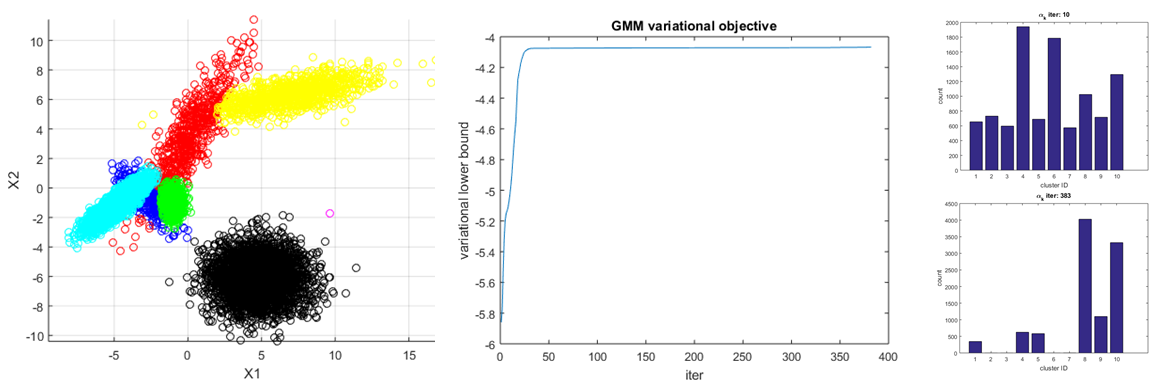
\includegraphics[width=0.8\textwidth, trim={10 10 10 10}]{figures/vb_gmm.png}
    \caption{Variational Bayes EM applied to a Mixture of Gaussians}
    \label{fig:vb_gmm}
\end{figure}

Figure \ref{fig:vb_gmm} shows the posterior clustering assignment as a result of running Variational Bayes EM algorithm on a Gaussian Mixture. The algorithm correctly identified $K=6$ clusters using $10$ clusters as the starting point. We can see the rapid increase in the variational objective when the algorithm figures out that it could increase the objective by removing unnecessary clusters in early iterations, while the plateau results in moving the clusters around. This is also evident from the prior and posterior parameter values for mixing proportions $\alpha_k$. As the number of iterations increase the counts for unnecessary mixture components drop to zero. 

\subsection{Application: Topic Models}

A topic model is a latent variable model for discrete data such as text documents. Latent Dirichlet Allocation (LDA) is a topic model that represents each document as a finite mixture of topics, where a topic is a distribution over words. The objective is to learn the shared topic distribution and topic proportions for each document. LDA assumes a bag of words model in which the words are exchangeable and as a result sentence structure is not preserved, i.e. only the word counts matter. Thus, each document is reduced to a vector of counts over the vocabulary $V$ and the entire corpus of $D$ documents is summarized in a \textit{term-document} matrix $A_{V\times D}$. LDA can be seen as a non-negative matrix factorization problem that takes the term-document matrix and factorizes it into a product of topics $W_{V\times K}$ and topic proportions $H_{K\times D}$: $A = WH$.\\

A common method for adjusting the word counts is \textit{tf-idf} that logarithmically drives down to zero word counts that occur frequently across documents: $A_{t,d} \log \frac{D}{n_t}$, where $D$ is the total number of documents in the corpus and $n_t$ is the number of documents where term $t$ appears. The \textit{tf-idf} smoothing identifies the sets of words that are discriminative for documents and leads to better model performance. The term-document matrix generalizes from counts of individual words (unigrams) to larger structural units such as $n$-grams. In the case of $n$-grams different smoothing techniques (such as Laplace smoothing) are used to address the lack of observations in a very large feature space.\\ 

\begin{figure}[tbhp]
    \centering
    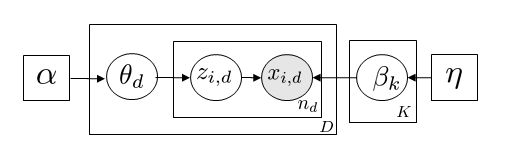
\includegraphics[width=0.5\textwidth, trim={10 10 10 10}]{figures/lda_gm.png}
    \caption{Latent Dirichlet Allocation (LDA) graphical model}
    \label{fig:lda_gm}
\end{figure}

Figure \ref{fig:lda_gm} shows the graphical model for the Latent Dirichlet Allocation (LDA). The LDA topic model associates each word $x_{i,d}$ with a topic label $z_{i,d} \in \{1,2,...,K\}$. Each document is associated with topic proportions $\theta_d$ that could be used to measure document similarity. The topics $\beta_k$ are shared across all documents. The hyper-parameters $\alpha$ and $\eta$ capture our prior knowledge of topic proportions and topics, respectively, e.g. from past on-line training of the model. The full generative model can be specified as follows:
\begin{eqnarray}
    \theta_d | \alpha &\sim& \mathrm{Dir}(\alpha)\\
    z_{i,d} | \theta_d &\sim& \mathrm{Cat}(\theta_d)\\
    \beta_k | \eta &\sim& \mathrm{Dir}(\eta)\\
    x_{i,d}|z_{i,d}=k,\beta &\sim& \mathrm{Cat}(\beta_k)
\end{eqnarray}
The joint distribution for a single document $d$ can be written as follows \cite{Blei2003}:
\begin{equation}
    p(x,z,\theta,|\alpha,\beta) = p(\theta_d|\alpha)\prod_{i=1}^{n_d}p(z_{i,d}|\theta_d)p(x_{i,d}|z_{i,d},\beta) 
\end{equation}
The parameters $\alpha$ and $\beta$ are corpus-level parameters, the variable $\theta_d$ is sampled once every document, while $z_{i,d}$ and $x_{i,d}$ are word-level variables sampled once for each word in each document. Unlike a multinomial clustering model where each document is associated with a single topic, LDA represents each document as a mixture of topics.\\

The key inference problem that we need to solve in order to use LDA is that of computing the posterior distribution of the latent variables for a given document: $p(\theta,z|x,\alpha,\beta)$. The posterior can be approximated with the following variational distribution:
\begin{equation}
    q(\theta,z|\gamma, \phi) = q(\theta|\gamma) \prod_{i=1}^{n}q(z_i|\phi_i)
\end{equation}
The variational parameters are optimized to maximize the Evidence Lower BOund (ELBO):
\begin{equation}
    \log p(x|\alpha,\eta) \geq L(x,\phi,\gamma,\lambda) = E_q[\log p(x,z,\theta,\beta|\alpha, \eta)] - E_q[\log q(z,\theta,\beta)] 
\end{equation}
We choose a fully factored distribution $q$ of the form:
\begin{equation}
    q(z_{id}=k)=\phi_{dwk}; ~~~ q(\theta_d) \sim \mathrm{Dir}(\theta_d|\gamma_d); ~~~ q(\beta_k) \sim \mathrm{Dir}(\beta_k|\lambda_k)
\end{equation}
We can expand the lower bound by using the factorizations of $p$ and $q$:
\begin{equation*}\label{equ:var1}
L(\gamma, \phi; \alpha, \beta) = \mathbb{E}_q [\log p(\theta|\alpha)] + \mathbb{E}_q [\log p(z|\theta)] + \mathbb{E}_q [\log p(w|z,\beta)] - \mathbb{E}_q[\log q(\theta)] - \mathbb{E}_q[\log q(z)]
\end{equation*}
Each of the five terms in $L(\gamma, \phi; \alpha, \beta)$ can be expanded \cite{Blei2003} as follows:
\begin{eqnarray}\label{equ:var2}
 L(\gamma, \phi; \alpha, \beta) &=& \log \Gamma(\sum_{j=1}^{k}\alpha_j) - \sum_{i=1}^{k}\log \Gamma(\alpha_i) + \sum_{i=1}^{k}(\alpha_i-1)(\Psi(\gamma_i)-\Psi(\sum_{j=1}^{k}\gamma_j)) \\
 &+& \sum_{n=1}^{N}\sum_{i=1}^{k}\phi_{ni}(\Psi(\gamma_i)-\Psi(\sum_{j=1}^{k}\gamma_j)) \\
 &+& \sum_{n=1}^{N}\sum_{i=1}^{k}\sum_{j=1}^{V}\phi_{ni}w_{n}^{j}\log \beta_{ij} \\
 &-& \log \Gamma(\sum_{j=1}^{k}\gamma_j) + \sum_{i=1}^{k}\log \Gamma(\gamma_i) - \sum_{i=1}^{k}(\gamma_i-1)(\Psi(\gamma_i)-\Psi(\sum_{j=1}^{k}\gamma_j)) \\
 &-& \sum_{n=1}^{N}\sum_{i=1}^{k}\phi_{ni}\log \phi_{ni} 
\end{eqnarray}
where $\Psi(x)=\frac{d}{dx}\log \Gamma(x)$ is the digamma function. $L(\gamma,\phi;\alpha,\beta)$ can be maximized using coordinate ascent over the variational parameters $\phi$, $\gamma$, $\lambda$ \cite{Blei2003}:
\begin{eqnarray}\label{equ:var3}
    \phi_{dwk} &\propto& \exp \{E_q[\log \theta_{dk}]+E_q[\log \beta_{kw}]\}\\
    \gamma_{dk} &=& \alpha + \sum_w n_{dw}\phi_{dwk} \\
    \lambda_{kw} &=& \eta + \sum_d n_{dw}\phi_{dwk}
\end{eqnarray}
where the expectations under $q$ of $\log \theta$ and $\log \beta$ are:
\begin{equation}
    E_q[\log \theta_{dk}] = \Psi(\gamma_{dk}) - \Psi(\sum_{i=1}^{K}\gamma_{di}) ~~~ E_q[\log \beta_{kw}] = \Psi(\lambda_{kw})-\Psi(\sum_{i=1}^{W}\lambda_{ki})
\end{equation}

The variational parameter updates in (\ref{equ:var3}) can be used in an online setting that does not require a full pass through the entire corpus at each iteration. An online update of variational parameters enables topic analysis for very large datasets including streaming data. Online VB for LDA is described in Algorithm \ref{alg:online_vb_lda}.\\

\begin{algorithm}
\caption{Online variational Bayes for LDA \cite{Hoffman2010}}
\label{alg:online_vb_lda}
\begin{algorithmic}[1]
\STATE Define $\rho_t = (\tau_0 + t)^{-\kappa}$
\STATE Initialize $\lambda$ randomly
\STATE for t = 1 to $\infty$ do 
\STATE ~~~ \textit{E step:} 
\STATE ~~~ Initialize $\gamma_{tk} = 1$ 
\STATE ~~~ \textbf{repeat} 
\STATE ~~~ ~~~ Set $\phi_{twk} \propto \exp \{E_q[\log \theta_{tk}]+E_q[\log \beta_{kw}]\}$ 
\STATE ~~~ ~~~ Set $\gamma_{tk} = \alpha + \sum_{w}\phi_{twk}n_{tw}$
\STATE ~~~ \textbf{until} $\frac{1}{K}\sum_k|\Delta \gamma_{tk}| < \epsilon$
\STATE ~~~ \textit{M step:} 
\STATE ~~~ Compute $\tilde{\lambda}_{kw} = \eta + Dn_{tw}\phi_{twk}$ 
\STATE ~~~ Set $\lambda = (1-\rho_t)\lambda + \rho_t \tilde{\lambda}$ 
\STATE end for
\end{algorithmic}
\end{algorithm}

As the $t$-th vector of word counts $n_t$ is observed, we perform an E step to find locally optimal values of $\gamma_t$ and $\phi_t$, holding $\lambda$ fixed. We then compute $\tilde{\lambda}$ that would be optimal if our entire corpus consisted of the single document $n_t$ repeated $D$ times. We then update $\lambda$ as a weighted average of its previous value and $\tilde{\lambda}$, where the weight is given by the learning parameter $\rho_t = (\tau_0 + t)^{-\kappa}$ for $\kappa \in (0.5,1]$, controlling the rate at which old values of $\tilde{\lambda}$ are forgotten.\\

\begin{figure}[tbhp]
    \centering
    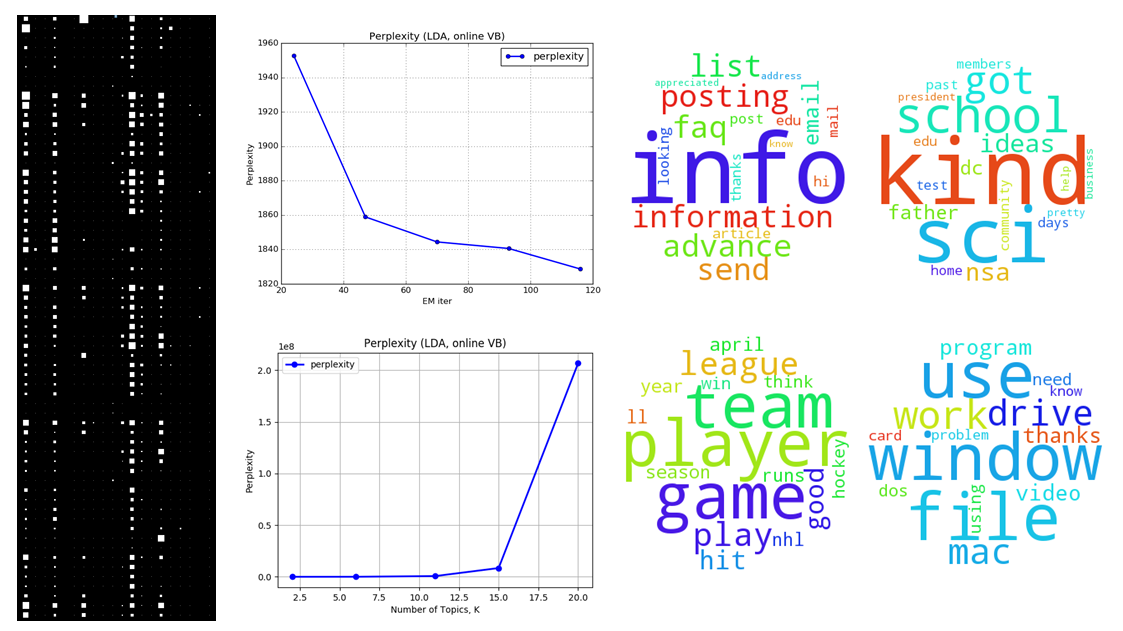
\includegraphics[width=0.8\textwidth, trim={10 10 10 10}]{figures/lda_onlinevb.png}
    \caption{Online Variational Bayes Inference Results for LDA.}
    \label{fig:lda_onlinevb}
\end{figure}

Figure \ref{fig:lda_onlinevb} shows the inference results for the online VB LDA algorithm on 20newsgroups dataset consisting of $11,314$ documents and a compressed vocabulary size of $1K$ words. The number of topics was set to $K=20$ and the batch size (number of documents to use in each EM iteration) was set to $512$. Figure \ref{fig:lda_onlinevb} shows the Hinton diagram of the inferred topic matrix $W_{V\times K}$ where only the first $64$ rows are shown. The perplexity plots show the improvement in model ability to explain the data as the number of EM iterations increases, where perplexity is defined as follows:
\begin{equation}\label{equ:perplexity1}
   \mathrm{Perplexity(w_{test})} = \exp\{-\frac{1}{D_{test}}\sum_{d} \frac{1}{n_d} \sum_{w \in n_d} \log p(w_{test})\}
\end{equation}
Model selection can be done by evaluating perplexity for different values of $K$. Guided by the fact that there are $20$ different newsgroups, the value of $K$ was set to $20$. Finally, the top $20$ words for a random sample of $4$ topics are shown in Figure \ref{fig:lda_onlinevb}. The four topics are about information, sports, computers and school.\\

\subsection{Stochastic Variational Inference}

One limitation of LDA is that the number of topics is fixed ahead of time. A commonly used approach to finding the number of topics $K$ is cross-validation. However, for very large data-sets this approach may not be practical. We can address this issue with a Bayesian non-parametric topic model where the number of topics is learned from data: the Hierarchical Dirichlet Process (HDP) topic model.




\section{Optimization}
\subsection{Simulated Annealing}

Simulated annealing is a stochastic algorithm that attempts to find the global optimum of an objective function $f(x)$. The method is inspired by statistical physics, in particular the Boltzmann distribution that specifies the probability of being in a particular state $x$:
\begin{equation}
    p(x) \propto \exp\{-f(x)/T\}
\end{equation}
where $f(x)$ is the energy of the system and $T$ is the temperature. As the temperature approaches zero, the system spends more and more time in its minimum energy (most probable) state. As the temperature decreases, the largest peaks become larger and the smallest peaks dissappear. By cooling slowly enough, it is possible to track the largest peak and therefore find the global optimum.\\

Simulated annealing is closely related to the Metropolis-Hastings algorithm for generating samples from a probability distribution. At each step of the algorithm, we sample a new state according to a proposal distribution $x^{\prime} \sim q(\dot|x_k)$, such as a random walk proposal:
\begin{equation}
    x^{\prime} = x_k + \epsilon_k, ~~~ \mathrm{where}~ \epsilon_k \sim N(0,\Sigma)
\end{equation}
Having proposed a new state, we compute $\alpha$ as in Algorithm \ref{alg:sim_annealing}.
\begin{algorithm}
\caption{Simulated Annealing}
\label{alg:sim_annealing}
\begin{algorithmic}[1]
\STATE $\alpha = \exp\{(f(x)-f(x^{\prime}))/T\}$
\STATE $r = \min(1,\alpha)$
\STATE $u \sim \mathrm{Unif}(0,1)$
\STATE if $u < r$ 
\STATE ~~~ $x_{k+1} = x^{\prime}$
\STATE else
\STATE ~~~ $x_{k+1} = x_k$
\STATE end if  
\end{algorithmic}
\end{algorithm}
Thus, if a new state has lower energy (higher probability), we will definitely accept it but if it has higher energy (lower probability), we might still accept it depending on the temperature. Therefore, the algorithm allows downhill moves in probability space but less frequently as the temperature drops. In practice it is common to use an exponential cooling schedule: $T_k = T_0 C^{k}$, where $T_0 \sim 1$ is the initial temperature and $C \sim 0.8$ is the cooling rate. Cooling too quickly can result in getting stuck in local optima, while cooling too slowly wastes time. The optimum cooling schedule is difficult to determine.    

\begin{figure}[tbhp]
    \centering
    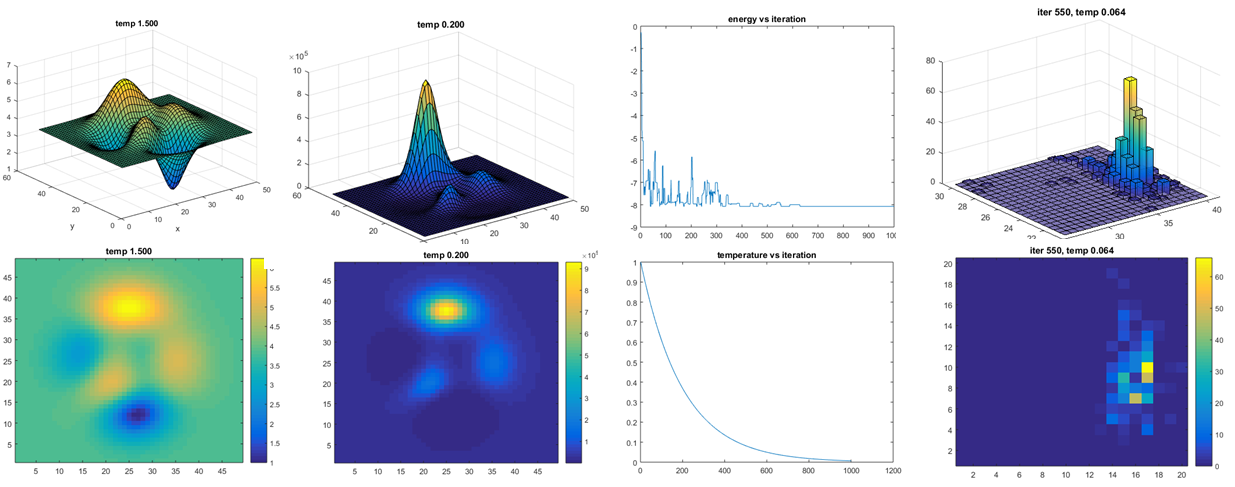
\includegraphics[width=0.9\textwidth, trim={10 10 10 10}]{figures/sim_annealing_merged.png}
    \caption{Simulated Annealing}
    \label{fig:sim_annealing_merged}
\end{figure}

Figure \ref{fig:sim_annealing_merged} shows the objective $f(x)$ at two different temperatures (left). The function appears more peaky when the temperature is lower. We can also see that the method stochastically reduces the energy over time for the given cooling schedule (middle). Finally a histogram of samples shows that most samples are concentrated near the global maximum (right).


\subsection{Bayesian Optimization}

Machine learning algorithms frequenty require careful tuning of hyperparameters. Often exhaustive and computationally expensive methods such as grid search cross validation are used to find model parameters that optimize a suitable performance objective. An alternative to grid search is randomized parameter optimization that samples parameter settings from a distribution over possible parameter values. This has two main benefits over the exhaustive search: the number of iterations can be chosen independent of the number of parameters and adding parameters that do not influence performance does not decrease efficiency. Rather than exploring the parameter space randomly (according to a chosen distribution), it would be great to adapt an active learning approach that selects parameter values in a way that reduces uncertainty and provides a balance between exploration and exploitation. Bayesian optimization provides an automated Bayesian framework by utilizing Gaussian Processes (GPs) to model algorithm's generalization performance \cite{snoek2012}.\\

Bayesian optimization assumes that a suitable performance function was sampled from a Gaussian Process and maintains a posterior distribution for this function as observations are made. To choose which hyperparameters to explore next, one can optimize the Expected Improvement (EI) over the current best result or the Gaussian process Upper Confidence Bound (UCB). EI and UCB have been shown to be efficient in the number of function evaluations required to find the global optimum of multi-modal black-box functions. Bayesian optimization uses all of the information available from previous evaluations of the objective function as opposed to relying on local gradient and Hessian approximations. This results in an automated procedure that can find an optimum of non-convex functions with relatively few evaluations, at the cost of performing more computation to determine the next point to try. This is particularly useful when evaluations are expensive to perform such as in selecting hyperparameters for deep neural networks.\\

To determine what point should be evaluated next, we need to choose and acquisition function which is used to construct a utility function from the GP posterior. In general, the acquisition function depends on previous observations as well as GP hyperparameters that we denote as $a(x;\{x_n,y_n\},\theta)$, then $x_{next} = \arg \max_x a(x)$. Let $\mu(x;\{x_n,y_n\},\theta)$ be the predictive GP mean function, $\sigma^{2}(x;\{x_n,y_n\},\theta)$ be the predictive GP variance function and $\Phi(x)$ be the cumulative distribution function of the standard normal. Then we can define the following acquisition functions.\\

\textit{Probability of Improvement}. This strategy maximizes the probability of improving over the best current value. This can be computed as follows:
\begin{equation}
    a_{PI}(x;\{x_n,y_n\},\theta) = \Phi(\gamma(x)), ~~~~ \gamma(x) = \frac{f(x_{best}) - \mu(x; \{x_n,y_n\},\theta)}{\sigma(x;\{x_n,y_n\},\theta)}
\end{equation}

\textit{Expected Improvement}. Alternatively, one could choose to maximize the expected improvement (EI) over the current best. 
\begin{equation}
    a_{EI}(x;\{x_n,y_n\},\theta) = \sigma(x;\{x_n,y_n\},\theta)(\gamma(x)\Phi(\gamma(x))+N(\gamma(x);0,1))
\end{equation}

\textit{Upper Confidence Bound}. UCB is the idea of exploiting upper confidence bounds to construct acquisition functions that minimize regret over the course of their optimization. These acquisition functions have the following form:
\begin{equation}
    a_{UCB}(x;\{x_n,y_n\},\theta) = \mu(x;\{x_n,y_n\},\theta) - \kappa \sigma(x;\{x_n,y_n\},\theta)
\end{equation}
where $\kappa$ is a tunable acquisition parameter to balance exploration and exploitation.\\


\begin{figure}[tbhp]
    \centering
    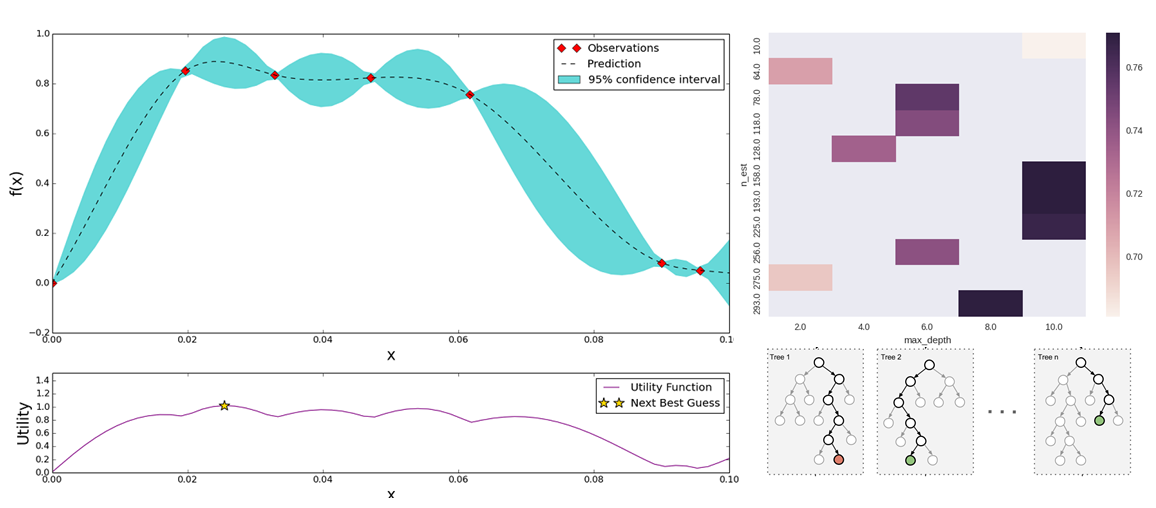
\includegraphics[width=0.95\textwidth, trim={10 10 10 10}]{figures/bayes_opt.png}
    \caption{Bayesian Optimization of SVM and Random Forest parameters}
    \label{fig:bayes_opt}
\end{figure}

Figure \ref{fig:bayes_opt} shows Baeysian optimization applied to SVM and Random Forest. F1 score was used as performance objective function for a classification task. The figure on the left shows Bayesian optimization of F1 score as a function of the gamma parameter of the SVM RBF kernel: $K(x,x^{\prime}) = \exp\{-\gamma ||x-x^{\prime}||^{2}\}$. We can see that after only 7 iterations we have discovered the gamma parameter that gives maximum F1 score. The peak of EI utility function at the bottom tells us which experiment to perform next. The figure on the right shows Bayesian optimization of F1 score as a function of maximum depth and the number of estimators of a Random Forest classifier. From the heatmap, we can tell that the maximum F1 score is achieved for $158$ estimators with depth equal to $10$.    


















\section{Misc}
\subsection{Sequential Monte Carlo}

Particle Filters (PF) is a Sequential Monte Carlo (SMC) method for estimating the internal states of a Switching Linear Dynamic System (SLDS). A set of particles is used to represent the posterior distribution of the states of the Markov process. At each iteration, the particles get re-samples and the ones that explain the observations best survive to the next iteration.

The Gaussian SLDS can be described as follows \cite{deFreitas2002}:
\begin{eqnarray}
    z_t &\sim& P(z_t | z_{t-1})\\
    x_t &=& A(z_t)x_{t-1} + B(z_t)w_t + F(z_t)u_t \\
    y_t &=& C(z_t)x_t + D(z_t)v_t + G(z_t)u_t
\end{eqnarray}
where $y_t \in \mathbb{R}$ denotes the observations, $x_t \in \mathbb{R}$ denotes latent Gaussian states, $z_t \in \mathbb{Z}$ denotes latent discrete states and $u_t$ is a known control signal. The noise processes are iid Gaussian with $w_t \sim N(0,I)$ and $v_t \sim N(0,I)$. This model implies the continuous densities:
\begin{eqnarray}\label{equ:smc_density}
    p(x_t|z_t,x_{t-1}) &\sim& N(A(z_t)x_{t-1} + F(z_t)u_t, B(z_t)B(z_t)^{T})\\
    p(y_t|x_t,z_t) &\sim& N(C(z_t)x_t + G(z_t)u_t, D(z_t)D(z_t)^{T})
\end{eqnarray}
along with initial states $x_0 \sim N(\mu_0,\Sigma_0)$ and $z_0 \sim P(z_0)$. The aim of the analysis is to compute the marginal posterior distribution of the discrete states $p(z_{0:t}, y_{1:t})$. The posterior density can be factorized as follows:
\begin{equation}
    p(x_{1:t},z_{1:t}|y_{1:t}) = p(x_{1:t}|y_{1:t},z_{1:t})p(z_{1:t}|y_{1:t})
\end{equation}
where the density $p(x_{1:t}|y_{1:t},z_{1:t})$ is Gaussian and can be computed analytically if we know the marginal posterior density $p(z_{1:t}|y_{1:t})$. We can re-write the marginal posterior recursively:
\begin{eqnarray}
   p(z_{1:t}|y_{1:t}) &=& \frac{p(y_t|z_{1:t}, y_{1:t-1})p(z_{1:t}|y_{1:t-1})}{p(y_t|y_{1:t-1})}\\
   &=& \frac{p(y_t|z_t)p(z_t|z_{1:t-1},y_{1:t-1})p(z_{1:t-1}|y_{1:t-1})}{p(y_t|y_{1:t-1})}\\
   &\propto& p(y_t|z_t)p(z_t|z_{t-1})p(z_{1:t-1}|y_{1:t-1})
\end{eqnarray}
which depends only on the current conditional distributions and previously computed $p(z_{1:t-1}|y_{1:t-1})$. The basic idea is to approximate the belief state of the entire state trajectory using a weighted set of particles:
\begin{equation}
    p(z_{1:t}|y_{1:t}) \approx \sum_{s=1}^{S}\hat{w}_{t}^{s}\delta_{z_{1:t}^{s}}(z_{1:t})
\end{equation}
We update this belief using importance sampling. If the proposal has the form $q(z_{1:t}^{s}|y_{1:t})$ then the importance weights are given by:
\begin{equation}
    w_{t}^{s} \propto \frac{p(z_{1:t}^{s}|y_{1:t})}{q(z_{1:t}^{s}|y_{1:t})} \propto \frac{p(y_t|x_t,z_t)p(x_t, z_t|x_{t-1},z_{t-1})}{q(x_t,z_t|x_{t-1},z_{t-1})} 
\end{equation}
We can choose the transition prior to be the proposal distribution:
\begin{equation}
     q(x_t,z_t|x_{t-1},z_{t-1}) = p(x_t, z_t|x_{t-1},z_{t-1}) = p(x_t|x_{t-1},z_{t-1})p(z_t|z_{t-1})
\end{equation}
then the importance weights are given by the likelihood function: $w_t \propto p(y_t|x_t,z_t)$. The particle filter algorithm is summarized in Algorithm \ref{alg:pf}.

\begin{algorithm}
\caption{Particle Filter Algorithm \cite{deFreitas2002}}
\label{alg:pf}
\begin{algorithmic}[1]
\STATE \textit{Sequential Importance Sampling Step}
\STATE for i = 1 to $N$ do  
\STATE ~~~ $z_{t}^{i} \sim p(z_t|z_{t-1}^{i})$ 
\STATE ~~~ $x_{t}^{i} \sim p(x_t|x_{t-1}^{i}, z_{t}^{i})$ as in eq. (\ref{equ:smc_density})
\STATE end for 
\STATE for i = 1 to $N$ do 
\STATE ~~~ $w_{t}^{i} \propto p(y_t|x_{t}^{i}, z_{t}^{i})$
\STATE end for
\STATE $\hat{w}_{t}^{i} = \frac{w_{t}^{i}}{\sum_{s^{\prime}}w_{t}^{s^{\prime}}}$ 
\STATE \textit{Selection Step}
\STATE ~~~ Multiply particles with respect to importance weights $w_{t}^{i}$
\STATE ~~~ to obtain $N$ particles $\{x_{1:t}^{i},z_{1:t}^{i}\}_{i=1}^{N}$
\STATE end for
\end{algorithmic}
\end{algorithm}

The selection step modifies the weighted approximate density $p_N$ to an unweighted density $\hat{p}_N$ by eliminating particles with low importance weights and by multiplying particles with high importance weights. Thus, $p_N(x)=\sum_{i=1}^{N}w_i\delta(x-x_i)$ is replaced by
\begin{equation}
    \hat{p}_N(x) = \sum_{k=1}^{N}\frac{1}{N}\delta(x-x_{k}^{\ast}) = \sum_{i=1}^{N}\frac{n_i}{N}\delta(x-x_i)
\end{equation}
There are many resampling schemes such as multinomial, stratified, systematic and residual.
All these algorithms are unbiased and can be implemented in $O(N)$ time.\\

The Rao-Blackwellized Particle Filter (RBPF) is similar to the PF but we only sample the discrete states. Then for each sample of the discrete states, we update the mean and covariance of the continuous states using Kalman filter updates. In particular, we sample $z_{t}^{i}$ and then propagate the mean $\mu_{t}^{i}$ and covariance $\Sigma_{t}^{i}$ of $x_t$ with a Kalman filter as follows:
\begin{eqnarray}
\mu_{t|t-1}^{i} &=& A(z_{t}^{i})\mu_{t-1|t-1}^{i} + F(z_{t}^{i})u_t\\
\Sigma_{t|t-1}^{i} &=& A(z_{t}^{i})\Sigma_{t-1|t-1}^{i}A(z_{t}^{i})^{T} + D(z_{t}^{i})D(z_{t}^{i})^{T}\\
S_{t}^{i} &=& C(z_{t}^{i})\Sigma_{t|t-1}^{i}C(z_{t}^{i})^{T} + D(z_{t}^{i})D(z_{t}^{i})^{T}\\
y_{t|t-1}^{i} &=& C(z_{t}^{i})\mu_{t|t-1}^{i} + G(z_{t}^{i})u_t\\
\mu_{t|t}^{i} &=& \mu_{t|t-1}^{i} + \Sigma_{t|t-1}^{i}C(z_{t}^{i})^{T}S_{t}^{-1}(y_t - y_{t|t-1}^{i})\\
\Sigma_{t|t}^{i} &=& \Sigma_{t|t-1}^{i} - \Sigma_{t|t-1}^{i}C(z_{t}^{i})^{T}S_{t}^{-1}C(z_{t}^{i})\Sigma_{t|t-1}^{i}
\end{eqnarray}

The RBPF takes slightly longer to compute but results in more accurate predictions. Figure \ref{fig:pf_merged} shows the generated SLDS states (left) and the inferred states (middle) by Particle Filter (PF) and the Rao-Blackwellized version (RBPF).
\begin{figure}[tbhp]
    \centering
    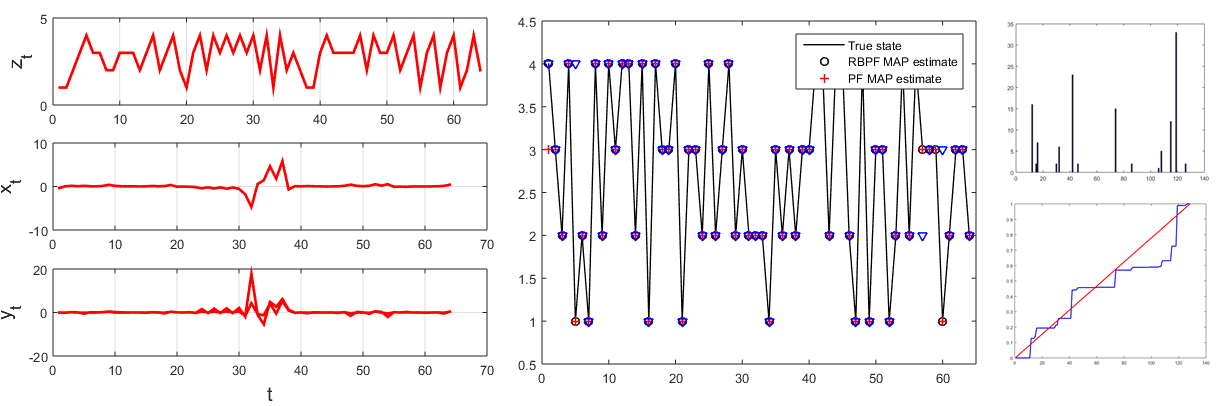
\includegraphics[width=0.9\textwidth, trim={10 10 10 10}]{figures/particle_filter_merged.png}
    \caption{Particle Filter inference using PF and RBPF applied to Switching Linear Dynamic System.}
    \label{fig:pf_merged}
\end{figure}
We can see that the inferred states closely correspond to the ground truth. Also shown is a particle resampling step (right) where only a fraction of the particles survive to the next iteration.


\subsection{Information Theory}

Information theory addresses the problems of data representation and reliable transmission of information. In order to measure information content, we define several information measures below.

\subsubsection{Entropy}

The entropy of a random variable is a measure of its uncertainty. Let $X$ be a discrete random variable with probability mass function $p(x)$, then its entropy is defined as:
\begin{equation}
    H(X) = -\sum_{x} p(x) \log p(x) = -E[\log p(x)]
\end{equation}
A maximum entropy discrete distribution is the uniform distribution. For a random variable with support $K$ and $p(x)=1/K$, the entropy is $H(X)= -\sum \frac{1}{K} \log \frac{1}{K} = \log_2 K$. Thus, entropy is measured in bits (using log base 2) or nats (using log base $e$). In contrast, the entropy of a deterministic random variable with $p(x) = \delta[x]$ is $H(X) = 1\log 1 = 0$. In the special case of a binary random variable $X \in \{0,1\}$ with $p(x=1)=p$, the entropy is
\begin{equation}
    H(X) = -p \log p - (1-p)\log (1-p)
\end{equation}
It is a concave function with maximum uncertainty of $1$ bit occuring at $p=\frac{1}{2}$, when $p=0$ or $p=1$, the entropy is $0$. Since entropy is a concave function on the space of distributions, we have:
\begin{equation}
    H(\lambda p_1 + (1-\lambda) p_2) \geq \lambda H(p_1) + (1-\lambda) H(p_2)
\end{equation}
Since $0\leq p(x) \leq 1$, we have $\log \frac{1}{p(x)} \geq 0$, and for a discrete $X$, the entropy is non-negative: $H(X)\geq 0$. We can find an upper bound for entropy using the Jensen's inequality:
\begin{eqnarray}
    H(X) &=& \sum_{x \in \cal X} p(x)\log \frac{1}{p(x)} \\
         &\leq& \log \sum_{x \in \cal X} p(x)\times \frac{1}{p(x)} \\
         &=& \log \sum_{x \in \cal X} 1 \\
         &=& \log |\cal X|
\end{eqnarray}
We also note that entropy is independent of permutation or cyclical shifts of the support of our distribution, i.e. it only depends on the point masses $p(x)$.\\

The joint entropy of a pair of discrete random variables $X$ and $Y$ is defined as:
\begin{equation}
    H(X,Y) = -\sum_x \sum_y p(x,y) \log p(x,y) = -E[\log p(x,y)]
\end{equation}
when two variables are independent the joint entropy is additivie: $H(X,Y) = H(X) + H(Y)$ iff $p(x,y) = p(x)p(y)$. The conditional entropy is defined as:
\begin{eqnarray}
    H(X|Y) &=& \sum_y p(y)H(X|Y=y) = -\sum_y p(y)\sum_x p(x|y)\log p(x|y) \\
           &=& -\sum_x \sum_y p(x,y)\log p(x|y) = -E[\log p(x|y)]
\end{eqnarray}
Note that conditioning on $Y$ the uncertainty over $X$ reduces on average: $H(X|Y) \leq H(X)$. The entropy of a pair of variables follows the chain rule:
\begin{eqnarray}
    H(X,Y) = H(X) + H(Y|X) = H(Y) + H(X|Y)
\end{eqnarray}
which follows from the chain rule for probability: $p(x,y) = p(x)p(y|x) = p(y)p(x|y)$. The chain rule can be generalized for multiple random variables $X_1,...,X_N$:
\begin{equation}
    H(X_1,...,X_N) = \sum_{i=2}^{N}H(X_i|X_1,...,X_{i-1}) + H(X_1) \leq \sum_{i=1}^{N} H(X_i)
\end{equation}
where the inequality follows from the fact that conditioning reduces entropy. For continuous random variables, the multivariate Gaussian is the distribution with maximum differential entropy:
\begin{eqnarray}
    h(X_1,...,X_N) &=& \int p(x) \log \frac{1}{p(x)} dx \\
    &=& \int p(x) \bigg[\frac{1}{2}\log (2\pi)^{d}|\Sigma| + \frac{1}{2}(x-\mu)^{T}\Sigma^{-1}(x-\mu)\bigg] dx \\
    &=& \frac{1}{2}\log (2\pi)^{d}|\Sigma| + \frac{1}{2}E[(x-\mu)^{T}\Sigma^{-1}(x-\mu)] \\
    &=& \frac{1}{2}\log (2\pi)^{d}|\Sigma| + \frac{1}{2}Tr\{\Sigma^{-1}\Sigma\} \\
    &=& \frac{1}{2}\log (2\pi)^{d}|\Sigma| + \frac{1}{2}d \log e = \frac{1}{2}\log\big[(2\pi e)^d|\Sigma|\big] 
\end{eqnarray}
In information theory, the analog of the law of large numbers is the Asymptotic Equipartition Property (AEP). The AEP states that:
\begin{theorem}
(AEP) If $X_1$,$X_2$,...,$X_n$ are iid $\sim p(x)$ then
\begin{equation}
    -\frac{1}{n} \log p(X_1, X_2,...,X_n) \rightarrow H(X) ~~~\mathrm{in~probability}
\end{equation}
\end{theorem}
\textit{Proof}.
\begin{equation}
    -\frac{1}{n}\log p(X_1, X_2,...,X_n) = -\frac{1}{n}\sum_i \log p(X_i) \rightarrow -E[\log p(X)] = H(X)
\end{equation}
Thus, the probability $p(X_1,...,X_n)$ assigned to an observed sequence will be close to $2^{-nH(X)}$. This enables us to classify the set of all sequences into a typical set, where the sample entropy is close to the true entropy and the nontypical set that contains all other sequences. 

\subsubsection{KL divergence}

One way to measure the similarity between two probability distributions $p(x)$ and $q(x)$ is the Kullback-Leibler divergence or relative entropy. It is defined as follows:
\begin{equation}
    KL(p||q) = \sum_x p(x) \log \frac{p(x)}{q(x)}
\end{equation}
we can re-write it as:
\begin{equation}
    KL(p||q) = \sum_x p(x)\log p(x) - \sum_x p(x)\log q(x) = -H(p) + H(p,q)
\end{equation}
where $H(p,q)$ is the cross-entropy. The regular entropy can be written as $H(p,p)$ and therefore KL divergence can be seen as a penalty of extra bits needed to encode the data due to the fact that we used a distribution $q(x)$ to represent the data instead of the true distribution $p(x)$. 
\begin{theorem}
 (Information Inequality) $KL(p||q)\geq 0$ with equality iff $p = q$. 
\end{theorem}
\textit{Proof}.
\begin{eqnarray}
    -KL(p||q) &=& -\sum_x p(x) \log \frac{p(x)}{q(x)} = \sum_x p(x)\log \frac{q(x)}{p(x)} \\
              &\leq& \log \sum_x p(x) \frac{q(x)}{p(x)} = \log \sum_x q(x)\\
              &\leq& \log 1 = 0
\end{eqnarray}
where we used the Jensen's inequality, which states that for any convex function $f(x)$, we have
\begin{equation}
    f\bigg(\sum_{i=1}^{n}\lambda_i x_i \bigg) \leq \sum_{i=1}^{n} \lambda_i f(x_i)
\end{equation}
where $\lambda_i \geq 0$ and $\sum_{i=1}^{n}\lambda_i = 1$.
However, KL divergence is not a true distance between distributions because it is not symmetric ($KL(p||q) \neq KL(q||p))$ and it does not satisfy the triangle inequality. We can use the information inequality to derive an upper bound on entropy. Let $u(x) = 1/|\cal X|$ be the uniform distribution, then:
\begin{eqnarray}
    0 &\leq& KL(p||u) = \sum_x p(x)\log \frac{p(x)}{u(x)} \\
      &=& \sum_x p(x)\log p(x) - \sum_x p(x)\log u(x) \\
      &=& -H(X) + \log |\cal X|
\end{eqnarray}
Thus, $H(X) \leq \log |\cal X|$ with equality iff $p(x) = u(x)$. 

\begin{theorem}
   $KL(p||q)$ is convex in the pair $(p,q)$, i.e.
   \begin{equation}
        KL(\lambda p_1 + (1-\lambda)p_2 || \lambda q_1 + (1-\lambda) q_2) \leq \lambda KL(p_1||q_1) + (1-\lambda) KL(p_2||q_2)
   \end{equation}
\end{theorem}
\textit{Proof}. Expanding the inequality above, we want to show that
\begin{eqnarray}
\sum_x(\lambda p_1(x) + (1-\lambda)p_2(x))\log\frac{\lambda p_1(x) + (1-\lambda)p_2(x)}{\lambda q_1(x) + (1-\lambda)q_2(x)} \leq \\
\lambda \sum_x p_1(x)\log\frac{p_1(x)}{q_1(x)} + (1-\lambda)\sum_x p_2(x)\log\frac{p_2(x)}{q_2(x)}
\end{eqnarray}
Then for a fixed $x$, it suffices to show that
\begin{equation}
    \sum_{i=1,2} \lambda_i p_i \log \frac{\lambda_i p_i}{\lambda_i q_i} \geq \bigg(\sum_{i=1,2}\lambda_i p_i \bigg)\bigg(\log \frac{\sum_i \lambda_i p_i}{\sum_i \lambda_i q_i} \bigg)
\end{equation}
where $\lambda_1 = \lambda$ and $\lambda_2 = 1-\lambda$, which is exactly the log-sum inequality.\\

In order to find a distribution $q(x) \in Q$ that is closest to $p(x) \in P$, we can minimize $KL(q||p)$ with respect to $q(x)$ known as I-projection or information projection:
\begin{equation}
    (\mathrm{I-projection}): ~~~ q(x) = \arg \min_{q \in Q} KL(q||p)
\end{equation}
Since the KL divergence is not symmetric in its arguments, the above expression will give different behavior compared to minimizing $KL(p||q)$ known as M-projection or moment projection:
\begin{equation}
    (\mathrm{M-projection}): ~~~ q(x) = \arg \min_{q \in Q} KL(p||q)
\end{equation}
Both the I-projection and the M-projection are projections of a probability distribution $p(x)$ onto a set of distributions $Q$. For I-projection, $q(x)$ will typically under-estimate the support of $p(x)$ and will lock onto one of its modes. This is due to $q(x)=0$ whenever $p(x)=0$ to make sure KL divergence stays finite. For M-projection, $q(x)$ will typically over-estimate the support of $p(x)$ and will cover all of its modes. This is due to $q(x)>0$ whenever $p(x)>0$ to make sure KL divergence stays finite. The I-projection is useful in setting up information geometry because of the following inequality:
\begin{equation}
    KL(q||p) \geq KL(q||p^{\ast}) + KL(p^{\ast}||p)
\end{equation}
The inequality can be interpreted as information-geometric version of Pythagoras' triangle inequality theorem, where KL divergernce is viewed as squared distance in Euclidean space.\\
If we are interested in measuring the distance between two multivariate Gaussian distributions with means $\mu_1$ and $\mu_2$ and covariances $\Sigma_1$ and $\Sigma_2$, the KL divergence can be computed in closed form:
\begin{eqnarray}
    KL(p||q) &=& \int p(x) \log \frac{p(x)}{q(x)} = \int [\log p(x) - \log q(x)] p(x) dx \nonumber \\
    &=& \int \bigg[\frac{1}{2}\log\frac{|\Sigma_2|}{|\Sigma_1|}-\frac{1}{2}(x-\mu_1)^{T}\Sigma_{1}^{-1}(x-\mu_1) + \frac{1}{2}(x-\mu_2)^{T}\Sigma_{2}^{-1}(x-\mu_2)\bigg]p(x) dx \nonumber \\
    &=& \frac{1}{2}\log\frac{|\Sigma_2|}{|\Sigma_1|}-\frac{1}{2}Tr\{E[(x-\mu_1)(x-\mu_1)^{T}\Sigma_{1}^{-1}]\} + \frac{1}{2}E[(x-\mu_2)^{T}\Sigma_{2}^{-1}(x-\mu_2)] \nonumber \\
    &=& \frac{1}{2}\log\frac{|\Sigma_2|}{|\Sigma_1|}-\frac{1}{2}Tr\{I_d\}+\frac{1}{2}(\mu_1-\mu_2)^{T}\Sigma_{2}^{-1}(\mu_1 - \mu_2) + \frac{1}{2}Tr\{\Sigma_{2}^{-1}\Sigma_1\} \nonumber \\
    &=& \frac{1}{2}\bigg[\log\frac{|\Sigma_2|}{|\Sigma_1|}-d+Tr(\Sigma_{2}^{-1}\Sigma_1)+(\mu_2-\mu_1)^{T}\Sigma_{2}^{-1}(\mu_2 - \mu_1) \bigg]
\end{eqnarray}


\subsubsection{Mutual Information}

Mutual information (MI) is a measure of overlap of random variables: amount of information one random variable contains about another random variable. Mutual information measures how similar the joint distribution $p(x,y)$ is compared to the factorized distribution $p(x)p(y)$ when the two variables are independent:
\begin{equation}
    I(X;Y) = KL(p(x,y)||p(x)p(y)) = \sum_x \sum_y p(x,y) \log \frac{p(x,y)}{p(x)p(y)}
\end{equation}
where $I(X;Y)\geq 0$ with equality iff the variables are independent: $p(x,y)=p(x)p(y)$. Mutual information between $X$ and $Y$ can be interpreted as the reduction in uncertainty about $X$ after observing $Y$ or by symmetry, the reduction in uncertainty about $Y$ after observing $X$:
\begin{equation}
    I(X;Y) = H(X) - H(X|Y) = H(Y) - H(Y|X) = H(X) + H(Y) - H(X,Y)
\end{equation}
\begin{figure}[tbhp]
    \centering
    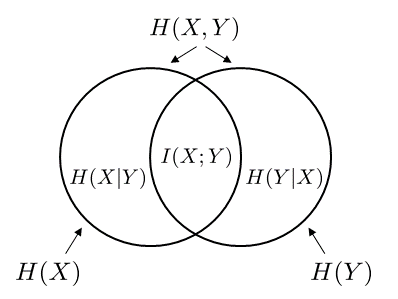
\includegraphics[width=0.4\textwidth, trim={10 10 10 10}]{figures/mutual_info.png}
    \caption{Relationship between entropy and mutual information}
    \label{fig:mutual_info}
\end{figure}
The relationship between entropy and MI is captured in a Venn diagram in Figure \ref{fig:mutual_info}. Note that entropy can be viewed as self-information $H(X) = I(X;X)$. The MI is the expected value of pointwise mutual information:
\begin{equation}
    PMI(x,y) = \log \frac{p(x,y)}{p(x)p(y)} = \log \frac{p(x|y)}{p(x)} = \log \frac{p(y|x)}{p(y)}
\end{equation}
This can be interpreted as the amount we learn from updating the prior $p(x)$ into the posterior $p(y|x)$
\begin{theorem}
(Data Processing Inequality). Let $X$, $Y$, $Z$ form the following Markov chain: $X\rightarrow Y\rightarrow Z$, then the following inequality holds:
\begin{equation}
    I(X;Y) \geq I(X;Z)
\end{equation}
\end{theorem}
\textit{Proof}. By the chain rule, we can expand mutual information in two different ways:
\begin{equation}
    I(X;Y,Z) = I(X;Z) + I(X;Y|Z) = I(X;Y) + I(X;Z|Y)
\end{equation}
Since $X$ is conditionally independent of $Z$ given $Y$, we have $I(X;Z|Y) = 0$ and therefore
\begin{equation}
    I(X;Y) = I(X;Z) + I(X;Y|Z)
\end{equation}
Since $I(X;Y|Z) \geq 0$, we have the inequality: $I(X;Y)\geq I(X;Z)$.
We can use the data processing inequality to show that \textit{sufficient statistics} preserves mutual information. In particular consider the data generating process: $\theta \rightarrow X \rightarrow T(X)$. Given distribution parameters $\theta$, we generate data by sampling from $f_{\theta}(x)$ and then we compute a statistic $T(X)$. The statistic $T(X)$ is called sufficient for $\theta$ if it contains all the information in $X$ about $\theta$, i.e. the data processing inequality is satisfied with equality:
\begin{equation}
    I(\theta; X) = I(\theta; T(X))
\end{equation}
Hence sufficient statistics compresses the information about $\theta$ using sampled data.\\

For a bivariate Gaussian distribution we can compute $I(X;Y)$ as follows.\\
Let $\rho = cov(X,Y)/\sigma_x \sigma_y$, and $\sigma^2 = var(X) = var(Y)$ then $h(X) = h(Y) = \frac{1}{2}\log(2\pi e)\sigma^2$ and
\begin{equation}
    h(X,Y) = \frac{1}{2}\log\big[(2\pi e)^{2}|\Sigma|\big] = \frac{1}{2}\log(2\pi e)^{2}\sigma^4(1-\rho^2)
\end{equation}
Therefore,
\begin{equation}
    I(X;Y) = h(X) + h(Y) - h(X,Y) = -\frac{1}{2}\log (1- \rho^2)
\end{equation}


\subsection{Imbalanced Learning}

Most classification algorithms will only perform optimally when the number of samples in each class is roughly the same. Highly skewed datasets where the minority class is outnumbered by one or more classes commonly occur in fraud detection, medical diagnosis and computational biology. One way of addressing this issue is by re-sampling the dataset to offset the imbalance and arrive at a more robust and accurate decision boundary. Re-sampling techniques can be broadly divided into four categories: undersampling the majority class, over-sampling the minority class, combining over and under sampling, and creating ensemble of balanced datasets \cite{He2009}.\\

\begin{figure}[tbhp]
    \centering
    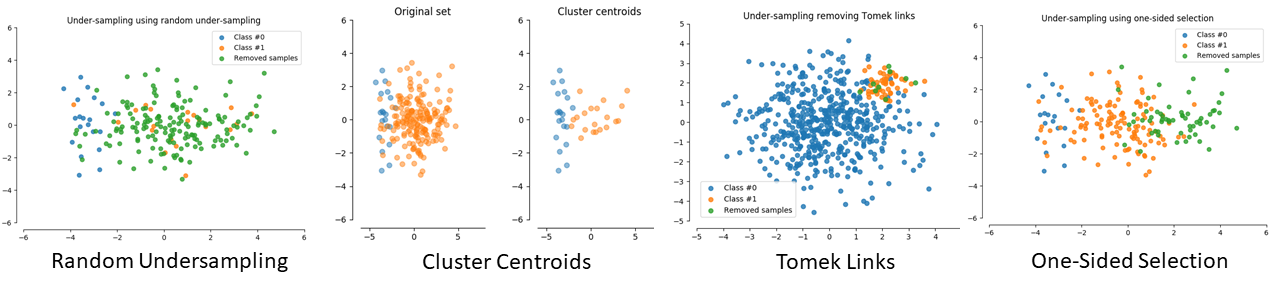
\includegraphics[width=0.95\textwidth, trim={10 10 10 10}]{figures/undersampling.png}
    \caption{Four undersampling strategies: random, cluster centroids, Tomek links, one-sided selection.}
    \label{fig:undersampling}
\end{figure}

\textit{Undersampling strategies}. Undersampling methods remove data from the majority class of the original dataset as shown in Figure \ref{fig:undersampling}. Random Under Sampler simply removes data points from the majority class uniformly at random. Cluster Centroids is a method that replaces cluster of samples by the cluster centroid of a K-means algorithm, where the number of clusters is set by the level of undersampling. Tomek links remove unwanted overlap between classes where Tomek links are removed until all minimally distanced nearest neighbor pairs are of the same class. A Tomek link is defined as follows: given an instance pair $(x_i, x_j)$, where $x_i \in S_{min}$, $x_j \in S_{maj}$ and $d(x_i,x_j)$ is the distance between $x_i$ and $x_j$, then the $(x_i, x_j)$ pair is called a Tomek link if there's no instance $x_k$ such that $d(x_i, x_k) < d(x_i, x_j)$ or $d(x_j, x_k) < d(x_i, x_j)$. In this way, if two instances form a Tomek link then either one of these instances is noise or both are near a border. Therefore one can use Tomek links to clean up overlap between classes. By removing overlapping examples, one can establish well-defined clusters in the training set and lead to improved classification performance. The One Sided Selection (OSS) method selects a representative subset of the majority class $E$ and combines it with the set of all minority examples $S_{min}$ to form $N = \{E\cup S_{min}\}$. The reduced set $N$ is further processed to remove all majority class Tomek links.\\  

\begin{figure}[tbhp]
    \centering
    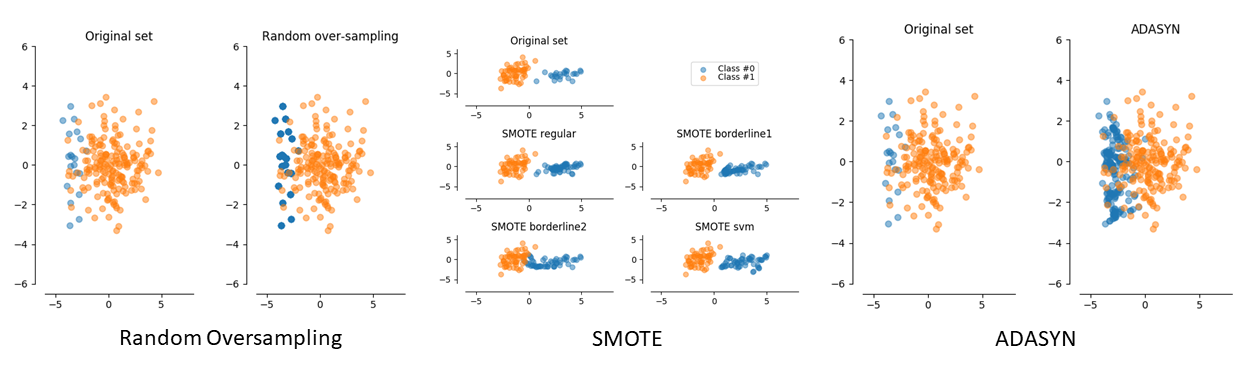
\includegraphics[width=0.95\textwidth, trim={10 10 10 10}]{figures/oversampling.png}
    \caption{Three oversampling strategies: random, SMOTE, ADASYN.}
    \label{fig:oversampling}
\end{figure}

\textit{Oversampling strategies}. Oversampling methods append data to the minority class of the original dataset as shown in Figure \ref{fig:oversampling}. Random Over Sampler simply adds data points to the minority class uniformly at random. Synthetic Minority Oversampling Technique (SMOTE) generates synthetic examples by finding $K$ nearest neighbors in the feature space and generating a new data point along the line segments joining any of the $K$ minority class nearest neighbors. Synthetic samples are generated in the following way: take the difference between the feature vector (sample) under consideration and its nearest neighbor, multiply this difference by a random number between $0$ and $1$ and add it to the feature vector under consideration thus augmenting the dataset with a new data point. Adaptive Synthetic Sampling (ADASYN) uses a weighted distribution for different minority class examples according to their level of difficulty in learning, where more synthetic data is generated for minority class examples that are harder to learn. As a result, the ADASYN approach improves learning of imbalanced dataset in two ways: reducing the bias introduced by class imbalance and adaptively shifting the classification decision boundary toward the difficult examples.\\ 

It's possible to combine over-sampling and under-sampling techniques into a hybrid strategy. Common examples include SMOTE and Tomek links or SMOTE and Edited Nearest Neighbors (ENN). Additional ways of learning on imbalanced datasets include weighing training instances, introducing different misclassification costs for positive and negative examples and bootstrapping. 







%\section{Experiments}
%The advantages of content-based superpixels are shown in several important vision tasks.

\subsection{Classification}

An AlexNet classifier trained on ImageNet data \cite{alex2012net} was used to classify images in the COCO dataset \cite{coco14data}. The superpixel centers were sampled from a Gaussian mixture centered at each region of interest (ROI) with equal proportions, while allocating $10\%$ of samples to background.

\begin{figure}[h]
	\centering
	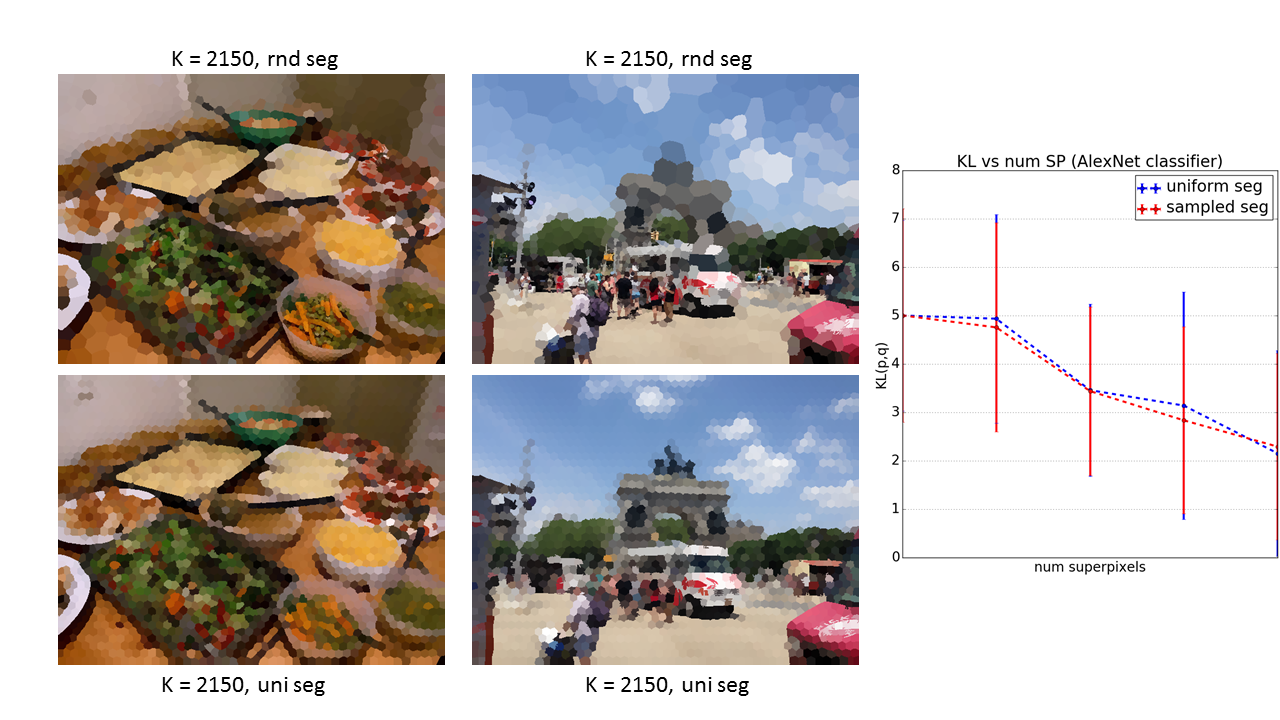
\includegraphics[width=0.8\textwidth, trim={10 10 10 10}]{figures/coco_merged.png}
	\caption{Top-row: content-based superpixels. Bottom-row: uniform superpixels. Right: KL divergence between classifier outputs.}
    \label{fig:coco}
\end{figure}

Figure \ref{fig:coco} shows the difference between content-based (top row) and uniform (bottom row) superpixels for sample images from the COCO dataset \cite{coco14data}. Also, shown on the right is the KL divergence of the output of AlexNex classifier in the two cases. We can see that the content-based superpixels are slightly lower compared to unifom superpixels.




\bibliographystyle{ieee}
\bibliography{research_journal}

\end{document}


